\section{Option Strategies}
\label{sect:option-strat}
\begin{enumerate}
\item In this section, we use the ``basic'' option positions: long call (LC),
long put (LP), short call (SC), and short put (SP), to ``compose'' more complex
option strategies.
\end{enumerate}
\subsection{Floors}
\label{subsect:floors}
\begin{enumerate}
\item A \emph{floor} is a strategy that insures a long position in an asset
\faIcon{apple-alt}.
\item P/L (at time \(T\)) graph for long \faIcon{apple-alt}:
\begin{center}
\begin{tikzpicture}[]
\begin{axis}[domain=0:5, ymin=-2.5, ymax=2.5, xmax=5.5, axis y line=left, axis x line=middle,
xtick={2.2}, ytick={-2.2}, title={Long \faIcon{apple-alt}},
xticklabel={\(S_0e^{rT}\)}, xticklabel style={xshift=0.3cm},
yticklabel={\(-S_0e^{rT}\)},
ylabel=P/L,
xlabel=\(S_T\),
ylabel style={at={(axis description cs:0,1)}, anchor=south, rotate=-90},
xlabel style={anchor=west}
]
\addplot[blue, thick]{x-2.2};
\node[red] at (1.5,-1.5) {risk \faIcon{exclamation-triangle}};
\draw[opacity=0.5, red, line width=0.2cm, line cap=round] (0,-2.2) -- (2.1,-0.1);
\end{axis}
\end{tikzpicture}
\end{center}
There is a risk for long \faIcon{apple-alt}: If the price of \faIcon{apple-alt}
drops \faIcon{chart-area} significantly after \(T\) years, we would suffer a
great loss.

\item To hedge (reduce) this risk \faIcon{shield-alt}, we can long a put on
\faIcon{apple-alt} since the ``initial positive'' part of the P/L graph for LP
can help reducing the risk:
\begin{center}
\begin{tikzpicture}[declare function={func(\x) = (\x <= 2) * (1.5-x) + (\x > 2) * -0.5;}]
\begin{axis}[domain=0:5, ymin=-2.5, ymax=2.5, xmax=5.5, axis y line=left, axis x line=middle,
xtick=\empty, ytick=\empty, samples=75,
ylabel=P/L,
ylabel style={at={(axis description cs:0,1)}, anchor=south, rotate=-90},
xlabel=\(S_T\),
xlabel style={anchor=west}, samples=75,
title=LP
]
\addplot[blue, thick]{func(x)};
\draw[opacity=0.4, ForestGreen, line width=0.2cm, line cap=round, line join=round] (0,1.5) -- (1.4,0.1);
\end{axis}
\end{tikzpicture}
\end{center}
This forms a \defn{floor} (long \faIcon{apple-alt} and LP):
\begin{center}
\begin{tikzpicture}[
declare function={
lp(\x) = (\x <= 2) * (1.5-x) + (\x > 2) * -0.5;
la(\x) = (x-2.2);
}
]
\begin{axis}[domain=0:5, ymin=-2.5, ymax=2.5, xmax=5.5, axis y line=left, axis x line=middle,
title={{\color{violet}Floor} = {\color{blue}Long \faIcon{apple-alt}} + {\color{orange}LP}},
xtick={2.2}, xticklabel={\(S_0e^{rT}\)}, xticklabel style={yshift=0.7cm, xshift=0.2cm},
ytick={-2.2},
yticklabel={\(-S_0e^{rT}\)},
ylabel=P/L,
ylabel style={at={(axis description cs:0,1)}, anchor=south, rotate=-90},
xlabel=\(S_T\),
xlabel style={anchor=west}, samples=75
]
\addplot[blue, thick, dashed, opacity=0.5]{la(x)};
\addplot[orange, thick, dashed, opacity=0.5]{lp(x)};
\addplot[violet, thick]{la(x)+lp(x)};
\draw[opacity=0.4, ForestGreen, line width=0.2cm, line cap=round, line join=round] (0,-0.7) -- (2,-0.7) -- (2.6,-0.1);
\node[ForestGreen] at (1.2,-0.4) {hedged \faIcon{shield-alt} risk};
\draw[-Latex] (3,-1) to[bend left] (1,-0.8);
\node[] () at (3.5,-0.8) {``Floor''};
\node[violet] () at (4,0.3) {slope = 1};
\end{axis}
\end{tikzpicture}
\end{center}
\item The P/L (at time \(T\)) of the (long) floor is given by
\[
\underbrace{S_T-S_0e^{rT}}_{\text{P/L of long \faIcon{apple-alt}}} +
\underbrace{(K-S_T)_{+}-P_0e^{rT}}_{\text{P/L of LP}}
=S_T+(K-S_T)_{+}-(S_0+P_0)e^{rT}.
\]
\item Based on the P/L of the floor and the no-arbitrage principle, it turns
out that we can derive a bound on the put option price \(P_0\). Consider the
payoff graph:
\begin{center}
\begin{tikzpicture}[
declare function={
lp(\x) = (\x <= 2) * (2-x) + (\x > 2) * 0;
la(\x) = (x);
}
]
\begin{axis}[domain=0:5, ymin=-2.5, xmax=5.5, axis y line=left, axis x line=middle,
xtick={2}, title={{\color{violet}Floor} = {\color{blue}Long \faIcon{apple-alt}} + {\color{orange}LP}},
xticklabel={\(K\)},
ytick={2},
yticklabel={\(K\)}, ylabel=Payoff, ylabel style={at={(axis description cs:0,1)}, anchor=south, rotate=-90},
xlabel=\(S_T\),
xlabel style={anchor=west}, samples=75
]
\addplot[blue, thick, dashed, opacity=0.5]{la(x)};
\addplot[orange, thick, dashed, opacity=0.5]{lp(x)};
\addplot[violet, thick]{la(x)+lp(x)};
\node[violet] () at (4,2.5) {slope = 1};
\end{axis}
\end{tikzpicture}
\end{center}
\begin{note}
The payoff of the floor is \(S_T+(K-S_T)_{+}\).
\end{note}

\item 
Let \(\pi_0\) be the time-0 price of the floor (which is \(S_0+P_0\)). Then,
its P/L can be expressed as
\[
S_T+(K-S_T)_{+}-\pi_0 e^{rT}.  \]
Since \(\pi_0 e^{rT}>0\) is a constant with respect to \(S_T\), the P/L graph
can also be obtained by shifting the payoff graph \emph{downward} by
\(\pi_0e^{rT}\):
\begin{center}
\begin{tikzpicture}[
declare function={
lp(\x) = (\x <= 2) * (2-x) + (\x > 2) * 0;
la(\x) = (x);
}
]
\begin{axis}[domain=0:5, ymin=-2.5, xmax=5.5, axis y line=left, axis x line=middle,
xtick={2}, title={{\color{violet}Floor} = Long \faIcon{apple-alt} + LP},
xticklabel={\(K\)},
ytick={2,-0.7},
yticklabels={\(K\),\(K-\pi_0e^{rT}\)}, ylabel=P/L, ylabel style={at={(axis description cs:0,1)}, anchor=south, rotate=-90},
xlabel=\(S_T\),
xlabel style={anchor=west}, samples=75
]
\addplot[violet, thick, dashed, opacity=0.3]{lp(x)+la(x)};
\addplot[violet, thick]{lp(x)+la(x)-2.7};
\draw[-Latex, brown] (0.8,1.8) -- (0.8,-0.5);
\draw[-Latex, brown] (1.6,1.8) -- (1.6,-0.5);
\draw[-Latex, brown] (2.4,2.2) -- (2.4,-0.1);
\draw[-Latex, brown] (3.2,3) -- (3.2,0.7);
\draw[-Latex, brown] (4,3.8) -- (4,1.5);
\node[brown] () at (4.8,3.3) {\(-\pi_0e^{rT}\)};
\node[violet] () at (4,0.3) {slope = 1};
\end{axis}
\end{tikzpicture}
\end{center}

\item \label{it:put-price-lb}
Under the no-arbitrage principle, the P/L cannot be always nonnegative. Hence,
we must have
\[
K-\pi_0 e^{rT}<0 \implies P_0>Ke^{-rT}-S_0,
\]
yielding a lower bound of the put option price \(P_0\).
\item The payoff graph of the floor has similar ``shape'' as the payoff graph
for \emph{long call}:
\begin{center}
\begin{tikzpicture}[scale=0.6, declare function={func(\x) = (\x <= 2) * 0 + (\x > 2) * (x-2);}]
\begin{axis}[domain=0:5, ymin=-2.5, ymax=2.5, xmax=5.5, axis y line=left, axis x line=middle,
xtick=\empty, ytick=\empty, samples=75]
\addplot[blue, thick]{func(x)};
\end{axis}
\end{tikzpicture}
\end{center}

\item \label{it:floor-lc-lb-payoff}
We can observe that the payoff graph of the floor can be obtained by
shifting the payoff graph of long call \emph{upward} by \(K\).

Indeed, the floor can also be ``composed'' using a \emph{long call} on
\faIcon{apple-alt} and a loan (lending \faIcon{dollar-sign} risk-free at time
0 such that a cash flow of \(K\) can be collected at time \(T\)).

\begin{note}
Sometimes the act of lending/borrowing \faIcon{dollar-sign} (risk-free) is
described as \emph{buying}/\emph{selling} a (risk-free zero-coupon) bond
\faIcon{scroll} \faIcon{arrow-right} having a \emph{long}/\emph{short} position
in bond \faIcon{scroll}.

The amount paid when buying the bond \faIcon{scroll} is the amount \emph{lent}
to the seller (borrower). Then, \faIcon{scroll} entitles its owner to later
collect proceeds from the bond seller.
\end{note}

To be more precise, we can ``decompose'' the payoff graph like below:

\begin{center}
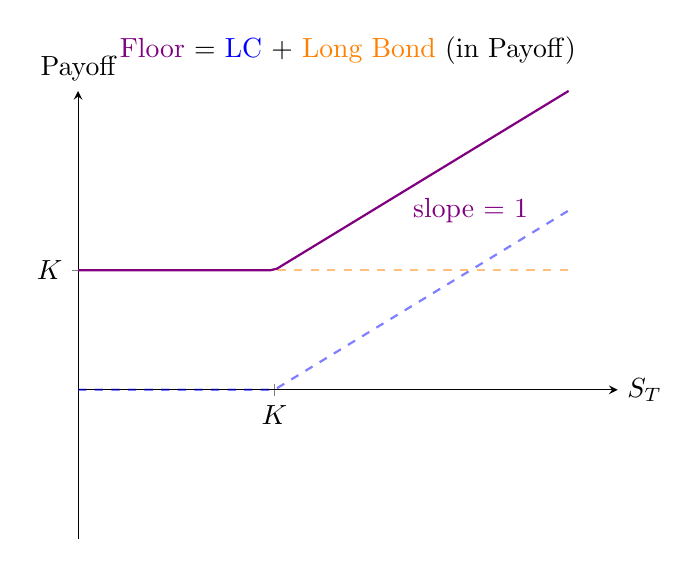
\begin{tikzpicture}[
declare function={
lc(\x) = (\x <= 2) * 0 + (\x > 2) * (\x - 2);
lb(\x) = 2;
}
]
\begin{axis}[domain=0:5, ymin=-2.5, xmax=5.5, axis y line=left, axis x line=middle,
xtick={2}, title={{\color{violet}Floor} = {\color{blue}LC} + {\color{orange}Long Bond} (in Payoff)},
xticklabel={\(K\)},
ytick={2},
yticklabel={\(K\)}, ylabel=Payoff, ylabel style={at={(axis description cs:0,1)}, anchor=south, rotate=-90},
xlabel=\(S_T\),
xlabel style={anchor=west}, samples=75
]
\addplot[blue, thick, dashed, opacity=0.5]{lc(x)};
\addplot[orange, thick, dashed, opacity=0.5]{lb(x)};
\addplot[violet, thick]{lb(x)+lc(x)};
\node[violet] () at (4,3) {slope = 1};
\end{axis}
\end{tikzpicture}
\end{center}
Algebraically we can write
\[
\underbrace{S_T+(K-S_T)_{+}}_{\text{floor payoff}}
=\underbrace{K+(S_T-K)_{+}}_{\mathclap{\text{``LC + long bond'' payoff}}},
\]
Since floor and ``LC + long bond'' have the same payoff, by the law of one
price, their (time-0) prices must be the same. (This yields the \emph{put-call
parity}; See \cref{subsect:put-call-parity}.)
\end{enumerate}
\subsection{Caps}
\begin{enumerate}
\item A \emph{cap} is a strategy that insures a short position in an asset \faIcon{apple-alt}.

\item P/L (at time \(T\)) graph for short \faIcon{apple-alt}:
\begin{center}
\begin{tikzpicture}[]
\begin{axis}[domain=0:5, ymin=-2.5, ymax=2.5, xmax=5.5, axis y line=left, axis x line=middle,
xtick={2.2}, ytick={2.2}, title={Short \faIcon{apple-alt}},
xticklabel={\(S_0e^{rT}\)}, xticklabel style={xshift=0.5cm, yshift=0.6cm},
yticklabel={\(S_0e^{rT}\)},
ylabel=P/L,
ylabel style={at={(axis description cs:0,1)}, anchor=south, rotate=-90},
xlabel=\(S_T\),
xlabel style={anchor=west}
]
\addplot[blue, thick]{2.2-x};
\node[red] at (4,-0.7) {risk \faIcon{exclamation-triangle}};
\draw[opacity=0.5, red, line width=0.2cm, line cap=round] (2.3,-0.1) -- (4.7,-2.5);
\end{axis}
\end{tikzpicture}
\end{center}
There is a risk for short \faIcon{apple-alt}: If the price of
\faIcon{apple-alt} rises \faIcon{chart-line} significantly after \(T\) years,
we would suffer a great loss.

\item To hedge this risk \faIcon{shield-alt}, we can long a call on
\faIcon{apple-alt} since the ``later positive'' part of the P/L graph for LC
can help reducing the risk:
\begin{center}
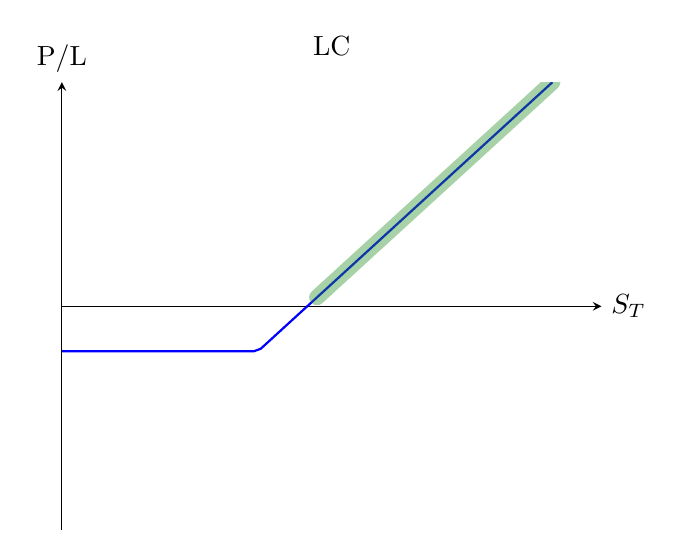
\begin{tikzpicture}[declare function={func(\x) = (\x <= 2) * (-0.5) + (\x > 2) * (\x-2.5);}]
\begin{axis}[domain=0:5, ymin=-2.5, ymax=2.5, xmax=5.5, axis y line=left, axis x line=middle,
xtick=\empty, ytick=\empty, samples=75,
ylabel=P/L,
ylabel style={at={(axis description cs:0,1)}, anchor=south, rotate=-90},
xlabel=\(S_T\),
xlabel style={anchor=west}, samples=75,
title=LC
]
\addplot[blue, thick]{func(x)};
\draw[opacity=0.4, ForestGreen, line width=0.2cm, line cap=round, line join=round] (2.6,0.1) -- (5,2.5);
\end{axis}
\end{tikzpicture}
\end{center}


This forms a \defn{cap} (short \faIcon{apple-alt} and LC):
\begin{center}
\begin{tikzpicture}[
declare function={
lc(\x) = (\x <= 2) * -0.5 + (\x > 2) * (\x-2.5);
sa(\x) = (2.2-\x);
}
]
\begin{axis}[domain=0:5, ymin=-2.5, ymax=2.5, xmax=5.5, axis y line=left, axis x line=middle,
title={{\color{violet}Cap} = {\color{blue}Short \faIcon{apple-alt}} + {\color{orange}LC}},
xtick={2.2}, xticklabel={\(S_0e^{rT}\)}, xticklabel style={yshift=0.6cm, xshift=0.5cm},
ytick={2.2},
yticklabel={\(S_0e^{rT}\)},
ylabel=P/L,
ylabel style={at={(axis description cs:0,1)}, anchor=south, rotate=-90},
xlabel=\(S_T\),
xlabel style={anchor=west}, samples=75
]
\addplot[blue, thick, dashed, opacity=0.5]{sa(x)};
\addplot[orange, thick, dashed, opacity=0.5]{lc(x)};
\addplot[violet, thick]{sa(x)+lc(x)};
\draw[opacity=0.4, ForestGreen, line width=0.2cm, line cap=round, line join=round] (1.8,-0.1) -- (2,-0.3) -- (5,-0.3);
\draw[-Latex] (3,-1.5) to[bend right] (4,-0.6);
\node[text width=4cm] () at (2,-1.5) {``Cap'' (cannot ``go down'' further)};
\node[violet] () at (2,0.7) {slope = \(-1\)};
\node[ForestGreen] at (2.8,-0.6) {hedged \faIcon{shield-alt} risk};
\end{axis}
\end{tikzpicture}
\end{center}
\item The P/L (at time \(T\)) of the cap is given by
\[
\underbrace{-S_T+S_0e^{rT}}_{\text{long \faIcon{apple-alt}}} +
\underbrace{(S_T-K)_{+}-C_0e^{rT}}_{\text{LC}}
=-S_T+(S_T-K)_{+}-(-S_0+C_0)e^{rT}.
\]
\item Similarly, based on the P/L of the cap and the no-arbitrage principle, we
can bound the call option price \(C_0\).  Consider the \emph{payoff}
graph:
\begin{center}
\begin{tikzpicture}[
declare function={
lc(\x) = (\x <= 2) * 0 + (\x > 2) * (\x-2);
sa(\x) = (-\x);
}
]
\begin{axis}[domain=0:5, ymin=-2.5, xmax=5.5, axis y line=left, axis x line=middle,
xtick={2}, title={{\color{violet}Cap} = {\color{blue}Short \faIcon{apple-alt}} + {\color{orange}LC}},
xticklabel={\(K\)},
ytick={-2},
yticklabel={\(-K\)}, ylabel=Payoff, ylabel style={at={(axis description cs:0,1)}, anchor=south, rotate=-90},
xlabel=\(S_T\),
xlabel style={anchor=west}, samples=75
]
\addplot[blue, thick, dashed, opacity=0.5]{sa(x)};
\addplot[orange, thick, dashed, opacity=0.5]{lc(x)};
\addplot[violet, thick]{sa(x)+lc(x)};
\node[violet] () at (2,-1) {slope = \(-1\)};
\end{axis}
\end{tikzpicture}
\end{center}
\begin{note}
The payoff of the cap is \(-S_T+(S_T-K)_{+}\).
\end{note}

\item \label{it:call-price-ub}
Let \(\pi_0\) be the time-0 price of the cap (which is \(-S_0+C_0\)). Then,
its P/L can be expressed as
\[
-S_T+(S_T-K)_{+}-\pi_0e^{rT}.
\]
Under the no-arbitrage principle, the P/L cannot be always nonpositive.
(Otherwise, \emph{reverse} cap would have an always nonnegative P/L
\faIcon{arrow-right} arbitrage!) Consequently, we need to shift the payoff
graph \emph{upward} to get the P/L graph. Hence, we have
\[
\pi_0<0\implies C_0<S_0,
\]
yielding an upper bound of the call option price \(C_0\).

\item The payoff graph of the cap has similar ``shape'' as the payoff graph for \emph{long
put}:
\begin{center}
\begin{tikzpicture}[scale=0.6, declare function={func(\x) = (\x <= 2) * (2-\x) + (\x > 2) * 0;}]
\begin{axis}[domain=0:5, ymin=-2.5, ymax=2.5, xmax=5.5, axis y line=left, axis x line=middle,
xtick=\empty, ytick=\empty, samples=75]
\addplot[blue, thick]{func(x)};
\end{axis}
\end{tikzpicture}
\end{center}

\item We can observe that the payoff graph of the cap can be obtained by
shifting the payoff graph of long put \emph{downward} by \(K\). So, the cap can
also be ``composed'' using a \emph{long put} on \faIcon{apple-alt} and a short
bond.

To be more precise, we can ``decompose'' the payoff graph like below:
\begin{center}
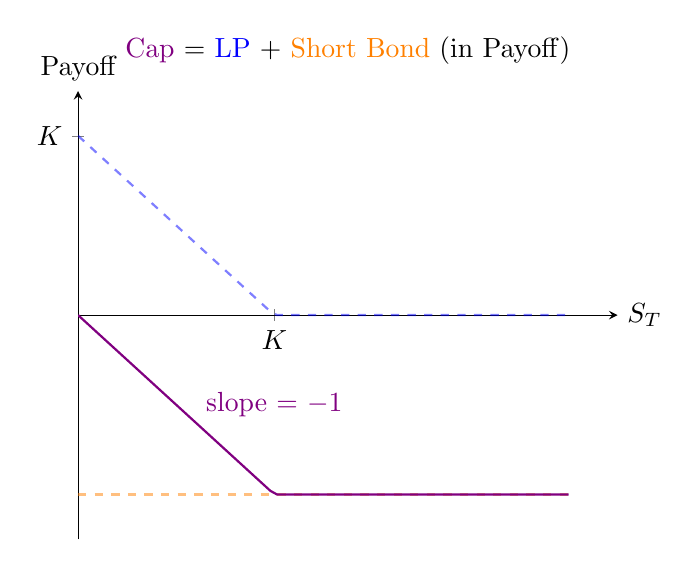
\begin{tikzpicture}[
declare function={
lp(\x) = (\x <= 2) * (2-\x) + (\x > 2) * 0;
sb(\x) = -2;
}
]
\begin{axis}[domain=0:5, ymin=-2.5, ymax=2.5, xmax=5.5, axis y line=left, axis x line=middle,
xtick={2}, title={{\color{violet}Cap} = {\color{blue}LP} + {\color{orange}Short Bond} (in Payoff)},
xticklabel={\(K\)},
ytick={2},
yticklabel={\(K\)}, ylabel=Payoff, ylabel style={at={(axis description cs:0,1)}, anchor=south, rotate=-90},
xlabel=\(S_T\),
xlabel style={anchor=west}, samples=75
]
\addplot[blue, thick, dashed, opacity=0.5]{lp(x)};
\addplot[orange, thick, dashed, opacity=0.5]{sb(x)};
\addplot[violet, thick]{sb(x)+lp(x)};
\node[violet] () at (2,-1) {slope = \(-1\)};
\end{axis}
\end{tikzpicture}
\end{center}
Algebraically we can write
\[
\underbrace{-S_T+(S_T-K)_{+}}_{\text{cap payoff}}
=\underbrace{-K+(K-S_T)_{+}}_{\mathclap{\text{``LP + short bond'' payoff}}},
\]
Since cap and ``LP + short bond'' have the same payoff, their (time-0) prices
must be the same by the law of one price.
\end{enumerate}
\subsection{Covered Calls}
\begin{enumerate}
\item P/L graph of writing a call on \faIcon{apple-alt}:
\begin{center}
\begin{tikzpicture}[declare function={func(\x) = (\x <= 2) * 0.5 + (\x > 2) * -(x-2.5);}]
\begin{axis}[domain=0:5, ymin=-3.5, ymax=1, xmax=5.5, axis y line=left, axis x line=middle,
xtick={2.5}, xticklabels={\(K+C_0e^{rT}\)}, xticklabel style={yshift=0.8cm, xshift=0.8cm},
ytick={0.5}, yticklabels={\(C_0e^{rT}\)}, ylabel=P/L,
ylabel style={at={(axis description cs:0,1)}, anchor=south, rotate=-90},
xlabel=\(S_T\),
xlabel style={anchor=west}, samples=75
]
\addplot[blue, thick]{func(x)};
\node[red] at (3,-1.5) {risk \faIcon{exclamation-triangle}};
\draw[opacity=0.5, red, line width=0.2cm, line cap=round] (2.6,-0.1) -- (5,-2.5);
\end{axis}
\end{tikzpicture}
\end{center}

\item To hedge this risk \faIcon{shield-alt}, we can long \faIcon{apple-alt}
since the ``later positive'' part of the P/L graph for long \faIcon{apple-alt}
can help reducing the risk:
\begin{center}
\begin{tikzpicture}[]
\begin{axis}[domain=0:5, ymin=-2.5, ymax=2.5, xmax=5.5, axis y line=left, axis x line=middle,
xtick={2.2}, ytick={-2.2}, title={Long \faIcon{apple-alt}},
xticklabel={\(S_0e^{rT}\)}, xticklabel style={xshift=0.3cm},
yticklabel={\(-S_0e^{rT}\)},
ylabel=P/L,
ylabel style={at={(axis description cs:0,1)}, anchor=south, rotate=-90},
xlabel=\(S_T\),
xlabel style={anchor=west}
]
\addplot[blue, thick]{x-2.2};
\draw[opacity=0.5, ForestGreen, line width=0.2cm, line cap=round] (2.3,0.1) -- (5,2.8);
\end{axis}
\end{tikzpicture}
\end{center}
\begin{remark}
\item The P/L graph of LC on \faIcon{apple-alt} also has a ``later positive''
part. But if we long a call on \faIcon{apple-alt}, we simply close out the
position, which is not so interesting.
\item ``Long forward on \faIcon{apple-alt}'' has the same P/L graph as
``long \faIcon{apple-alt}'', so long forward is not that much ``different''
from long \faIcon{apple-alt}. Still, we shall consider long \faIcon{apple-alt}
here.
\end{remark}
The act of writing the call \emph{together with} long \faIcon{apple-alt} is
known as \emph{writing}/\emph{selling} a \defn{covered call} (on
\faIcon{apple-alt}). In other words,
\[
\text{short covered call} = \text{short call} + \text{long \faIcon{apple-alt}}.
\]
\begin{note}
In contrast with \emph{writing a covered call} on \faIcon{apple-alt}, the act
of writing a call on \faIcon{apple-alt} without having any position in
\faIcon{apple-alt} simultaneously is known as \emph{writing} a \defn{naked
call} (or \defn{uncovered call}).  (``Naked'' and ``uncovered'' have
``similar'' meaning.)
\end{note}
\item The P/L graph of short covered call is:
\begin{center}
\begin{tikzpicture}[
declare function={
sc(\x) = (\x <= 2) * 0.5 + (\x > 2) * -(\x-2.5);
la(\x) = (\x-2.2);
}
]
\begin{axis}[domain=0:5, ymin=-2.5, ymax=2.5, xmax=5.5, axis y line=left, axis x line=middle,
title={{\color{violet}Short Covered Call} = {\color{blue}SC} + {\color{orange}Long \faIcon{apple-alt}}}, xtick={2.5}, xticklabels={\(K+C_0e^{rT}\)},
ytick={0.5}, yticklabels={\(C_0e^{rT}\)},
ylabel=P/L,
ylabel style={at={(axis description cs:0,1)}, anchor=south, rotate=-90},
xlabel=\(S_T\),
xlabel style={anchor=west}, samples=75
]
\addplot[blue, thick, dashed, opacity=0.5]{sc(x)};
\addplot[orange, thick, dashed, opacity=0.5]{la(x)};
\addplot[violet, thick]{sc(x)+la(x)};
\draw[opacity=0.4, ForestGreen, line width=0.2cm, line cap=round, line join=round] (2.6,0.3) -- (5,0.3);
\draw[-Latex, dashed, ForestGreen] (4,-1.3) to[bend right] (4.5,0.2);
\node[ForestGreen] at (4.5,-0.7) {eliminated risk};
\draw[opacity=0.4, red, line width=0.2cm, line cap=round, line join=round] (0.1,-1.6) -- (1.6,-0.1);
\node[red, text width=2cm] at (1.6,-1.3) {risk \faIcon{exclamation-triangle} (side effect)};
\end{axis}
\end{tikzpicture}
\end{center}
We can note that \emph{another} risk is created as a side effect,
unfortunately. However, as this risk is now ``limited'' (unlike the unlimited
potential loss for SC), the situation may be said to be ``improved''.  (In some
sense, we are ``exchanging'' the risk we face for  another kind of risk.)
\item The P/L of the short covered call is
\[
\underbrace{-(S_T-K)_{+}+C_0e^{rT}}_{\text{SC}}+\underbrace{S_T-S_0e^{rT}}_{\text{long \faIcon{apple-alt}}}
=S_T-(S_T-K)_{+}+(C_0-S_0)e^{rT}.
\]
\item Now, consider its payoff graph:
\begin{center}
\begin{tikzpicture}[
declare function={
sc(\x) = (\x <= 2) * 0 + (\x > 2) * -(\x-2);
la(\x) = (\x);
}
]
\begin{axis}[domain=0:5, ymin=-2.5, ymax=2.5, xmax=5.5, axis y line=left, axis x line=middle,
title={{\color{violet}Short Covered Call} = {\color{blue}SC} + {\color{orange}Long \faIcon{apple-alt}}},
xtick={2}, xticklabels={\(K\)},
ytick=\empty,
ylabel=Payoff,
ylabel style={at={(axis description cs:0,1)}, anchor=south, rotate=-90},
xlabel=\(S_T\),
xlabel style={anchor=west}, samples=75
]
\addplot[blue, thick, dashed, opacity=0.5]{sc(x)};
\addplot[orange, thick, dashed, opacity=0.5]{la(x)};
\addplot[violet, thick]{sc(x)+la(x)};
\end{axis}
\end{tikzpicture}
\end{center}
The ``shape'' of the graph looks like the one for the payoff graph for SP:

\begin{center}
\begin{tikzpicture}[scale=0.6, declare function={func(\x) = (\x <= 2) * -(2-\x) + (\x > 2) * 0;}]
\begin{axis}[domain=0:5, ymin=-2.5, ymax=2.5, xmax=5.5, axis y line=left, axis x line=middle,
xtick=\empty, ytick=\empty, samples=75]
\addplot[blue, thick]{func(x)};
\end{axis}
\end{tikzpicture}
\end{center}

Indeed, short covered call shares the same payoff as ``SP + long bond'' (hence
they have the same time-0 value):
\begin{center}
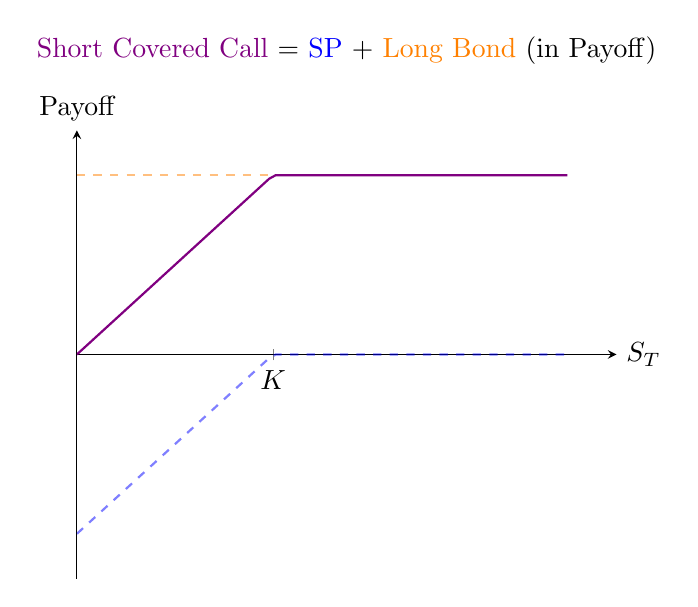
\begin{tikzpicture}[
declare function={
sp(\x) = (\x <= 2) * -(2-x) + (\x > 2) * 0;
lb(\x) = 2;
}
]
\begin{axis}[domain=0:5, ymin=-2.5, ymax=2.5, xmax=5.5, axis y line=left, axis x line=middle,
title={{\color{violet}Short Covered Call} = {\color{blue}SP} + {\color{orange}Long Bond} (in Payoff)},
title style={yshift=0.5cm},
xtick={2}, xticklabels={\(K\)},
ytick=\empty,
ylabel=Payoff,
ylabel style={at={(axis description cs:0,1)}, anchor=south, rotate=-90},
xlabel=\(S_T\),
xlabel style={anchor=west}, samples=75
]
\addplot[blue, thick, dashed, opacity=0.5]{sp(x)};
\addplot[orange, thick, dashed, opacity=0.5]{lb(x)};
\addplot[violet, thick]{sp(x)+lb(x)};
\end{axis}
\end{tikzpicture}
\end{center}
\end{enumerate}

\subsection{Covered Puts}
\begin{enumerate}
\item P/L graph of writing a put on \faIcon{apple-alt}:
\begin{center}
\begin{tikzpicture}[declare function={func(\x) = (\x <= 2) * -(1.5-x) + (\x > 2) * 0.5;}]
\begin{axis}[domain=0:5, ymin=-3.5, ymax=1, xmax=5.5, axis y line=left, axis x line=middle,
xtick={1.5}, xticklabels={\(K-P_0e^{rT}\)}, xticklabel style={yshift=0.8cm, xshift=-0.5cm},
ytick={0.5}, yticklabels={\(P_0e^{rT}\)}, ylabel=P/L,
ylabel style={at={(axis description cs:0,1)}, anchor=south, rotate=-90},
xlabel=\(S_T\),
xlabel style={anchor=west}, samples=75, title=Short Put
]
\addplot[blue, thick]{func(x)};
\draw[opacity=0.4, red, line width=0.2cm, line cap=round, line join=round] (0.1,-1.4) -- (1.4,-0.1);
\node[red] at (1.2,-1) {risk \faIcon{exclamation-triangle}};
\end{axis}
\end{tikzpicture}
\end{center}

\item In a similar manner, to hedge this risk \faIcon{shield-alt}, we can short
\faIcon{apple-alt} since the ``initial positive'' part of the P/L graph for
``short \faIcon{apple-alt}'' can help reducing the risk:
\begin{center}
\begin{tikzpicture}[]
\begin{axis}[domain=0:5, ymin=-2.5, ymax=2.5, xmax=5.5, axis y line=left, axis x line=middle,
xtick={2.2}, ytick={2.2}, title={Short \faIcon{apple-alt}},
xticklabel={\(S_0e^{rT}\)}, xticklabel style={xshift=-0.3cm},
yticklabel={\(S_0e^{rT}\)},
ylabel=P/L,
ylabel style={at={(axis description cs:0,1)}, anchor=south, rotate=-90},
xlabel=\(S_T\),
xlabel style={anchor=west}
]
\addplot[blue, thick]{2.2-x};
\draw[opacity=0.5, ForestGreen, line width=0.2cm, line cap=round] (0.1,2.1) -- (2.1,0.1);
\end{axis}
\end{tikzpicture}
\end{center}
Likewise, \emph{writing} a \defn{covered put} (on \faIcon{apple-alt}) means
writing a put on \faIcon{apple-alt} together with short \faIcon{apple-alt},
i.e.,
\[
\text{short covered put} = \text{short put} + \text{short \faIcon{apple-alt}}.
\]
\begin{note}
In contrast with \emph{writing a covered put} on \faIcon{apple-alt}, the act of
writing a put on \faIcon{apple-alt} without having any position in
\faIcon{apple-alt} simultaneously is known as \emph{writing} a \defn{naked put}
(or \defn{uncovered put}).
\end{note}
\item The P/L graph of short covered put is:
\begin{center}
\begin{tikzpicture}[
declare function={
sp(\x) = (\x <= 2) * -(1.5-\x) + (\x > 2) * 0.5;
sa(\x) = (2.2-\x);
}
]
\begin{axis}[domain=0:5, ymin=-2.5, ymax=2.5, xmax=5.5, axis y line=left, axis x line=middle,
title={{\color{violet}Short Covered Put} = {\color{blue}SP} + {\color{orange}Short \faIcon{apple-alt}}},
xtick={1.5}, xticklabels={\(K-P_0e^{rT}\)}, xticklabel style={yshift=0.7cm},
ytick={0.5}, yticklabels={\(P_0e^{rT}\)},
ylabel=P/L,
ylabel style={at={(axis description cs:0,1)}, anchor=south, rotate=-90},
xlabel=\(S_T\),
xlabel style={anchor=west}, samples=75
]
\addplot[blue, thick, dashed, opacity=0.5]{sp(x)};
\addplot[orange, thick, dashed, opacity=0.5]{sa(x)};
\addplot[violet, thick]{sp(x)+sa(x)};
\draw[opacity=0.4, ForestGreen, line width=0.2cm, line cap=round, line join=round] (0.1,0.7) -- (1.4,0.7);
\draw[-Latex, dashed, ForestGreen] (0.7,-0.7) to[bend left] (0.9,0.6);
\node[ForestGreen] at (0.6,-0.3) {elim.\ risk};
\draw[opacity=0.4, red, line width=0.2cm, line cap=round, line join=round] (2.8,-0.1) -- (5,-2.3);
\node[red] at (2.3,-1.3) {risk \faIcon{exclamation-triangle} (side effect)};
\end{axis}
\end{tikzpicture}
\end{center}
Since the risk in fact changes from \emph{limited} (SP) to \emph{unlimited}
(here), the situation may be seen as ``worsened'' unfortunately. Thus, we
seldom write covered put in practice.

\item Now, consider its payoff graph:
\begin{center}
\begin{tikzpicture}[
declare function={
sp(\x) = (\x <= 2) * -(2-\x) + (\x > 2) * 0;
sa(\x) = (-\x);
}
]
\begin{axis}[domain=0:5, ymax=2.5, xmax=5.5, axis y line=left, axis x line=middle,
title={{\color{violet}Short Covered Put} = {\color{blue}SP} + {\color{orange}Short \faIcon{apple-alt}}},
xtick={2}, xticklabels={\(K\)}, xticklabel style={yshift=0.7cm},
ytick=\empty,
ylabel=Payoff,
ylabel style={at={(axis description cs:0,1)}, anchor=south, rotate=-90},
xlabel=\(S_T\),
xlabel style={anchor=west}, samples=75
]
\addplot[blue, thick, dashed, opacity=0.5]{sp(x)};
\addplot[orange, thick, dashed, opacity=0.5]{sa(x)};
\addplot[violet, thick]{sp(x)+sa(x)};
\end{axis}
\end{tikzpicture}
\end{center}
The ``shape'' of the graph looks like the payoff graph for SC:

\begin{center}
\begin{tikzpicture}[scale=0.6, declare function={func(\x) = (\x <= 2) * 0 + (\x > 2) * -(\x-2);}]
\begin{axis}[domain=0:5, ymin=-2.5, ymax=2.5, xmax=5.5, axis y line=left, axis x line=middle,
xtick=\empty, ytick=\empty, samples=75]
\addplot[blue, thick]{func(x)};
\end{axis}
\end{tikzpicture}
\end{center}

Similarly, we can note that short covered put has the same payoff as ``SC +
short bond'' (so they have the same time-0 value):
\begin{center}
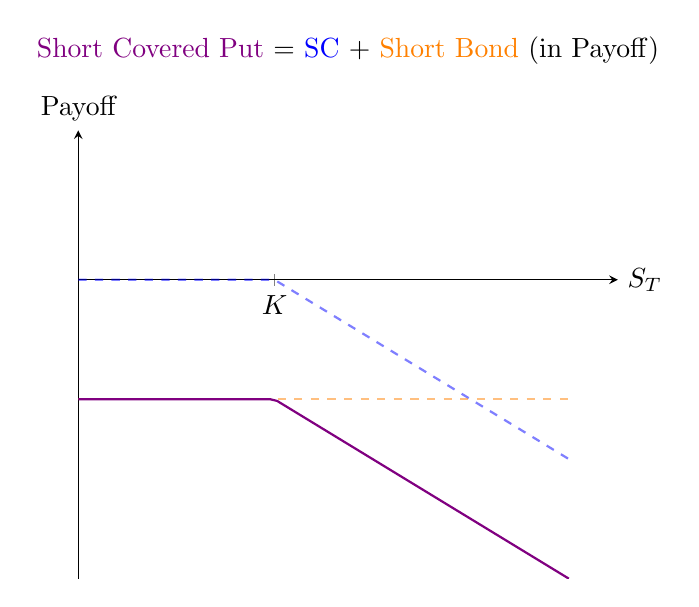
\begin{tikzpicture}[
declare function={
sc(\x) = (\x <= 2) * 0 + (\x > 2) * -(x-2);
sb(\x) = -2;
}
]
\begin{axis}[domain=0:5, ymax=2.5, xmax=5.5, axis y line=left, axis x line=middle,
title={{\color{violet}Short Covered Put} = {\color{blue}SC} + {\color{orange}Short Bond} (in Payoff)},
title style={yshift=0.5cm},
xtick={2}, xticklabels={\(K\)},
ytick=\empty,
ylabel=Payoff,
ylabel style={at={(axis description cs:0,1)}, anchor=south, rotate=-90},
xlabel=\(S_T\),
xlabel style={anchor=west}, samples=75
]
\addplot[blue, thick, dashed, opacity=0.5]{sc(x)};
\addplot[orange, thick, dashed, opacity=0.5]{sb(x)};
\addplot[violet, thick]{sc(x)+sb(x)};
\end{axis}
\end{tikzpicture}
\end{center}
\end{enumerate}
\subsection{Synthetic Forwards}
\label{subsect:synthetic-fwd}
\begin{enumerate}
\item Recall that a call/put option on \faIcon{apple-alt} gives its holder the
\emph{right} (but not the obligation) to buy/sell \faIcon{apple-alt}. But it
turns out by \emph{combining} two option positions, we can convert the
``rights'' to an \emph{obligation} (forming a \emph{synthetic forward} which
mimics a \emph{forward}).
\item To construct a synthetic forward, consider the payoff graphs of the four
``basic'' options (LC, LP, SC, SP) on \faIcon{apple-alt} (all with strike price
\(K\)):
\begin{center}
\begin{tikzpicture}[scale=0.4, declare function={func(\x) = (\x <= 2) * 0 + (\x > 2) * (x-2);}]
\begin{axis}[domain=0:5, ymin=-2.5, ymax=2.5, xmax=5.5, axis y line=left, axis x line=middle,
xtick=\empty, ytick=\empty, samples=75, title=\Huge{LC}]
\addplot[blue, thick]{func(x)};
\end{axis}
\end{tikzpicture}
\begin{tikzpicture}[scale=0.4, declare function={func(\x) = (\x <= 2) * (2-x) + (\x > 2) * 0;}]
\begin{axis}[domain=0:5, ymin=-2.5, ymax=2.5, xmax=5.5, axis y line=left, axis x line=middle, xtick=\empty, ytick=\empty, samples=75, title=\Huge{LP}]
\addplot[blue, thick]{func(x)};
\end{axis}
\end{tikzpicture}
\begin{tikzpicture}[scale=0.4, declare function={func(\x) = (\x <= 2) * 0 + (\x > 2) * -(x-2);}]
\begin{axis}[domain=0:5, ymin=-2.5, ymax=2.5, xmax=5.5, axis y line=left, axis x line=middle,
xtick=\empty, ytick=\empty, samples=75, title=\Huge{SC}]
\addplot[blue, thick]{func(x)};
\end{axis}
\end{tikzpicture}
\begin{tikzpicture}[scale=0.4, declare function={func(\x) = (\x <= 2) * -(2-x) + (\x > 2) * 0;}]
\begin{axis}[domain=0:5, ymin=-2.5, ymax=2.5, xmax=5.5, axis y line=left, axis x line=middle,
xtick=\empty, ytick=\empty, samples=75, title=\Huge{SP}]
\addplot[blue, thick]{func(x)};
\end{axis}
\end{tikzpicture}
\end{center}
Since the payoff of a long (short) forward is upward (downward) sloping, a
synthetic long (short) forward by combining option positions with ``upward
(downward) sloping'' parts, i.e.,
\begin{itemize}
\item \defn{synthetic long forward} (@ \(K\)) = LC (@ \(K\)) + SP (@ \(K\));
\item \defn{synthetic short forward} (@ \(K\)) = SC (@ \(K\))+ LP (@ \(K\)).
\end{itemize}

\begin{center}
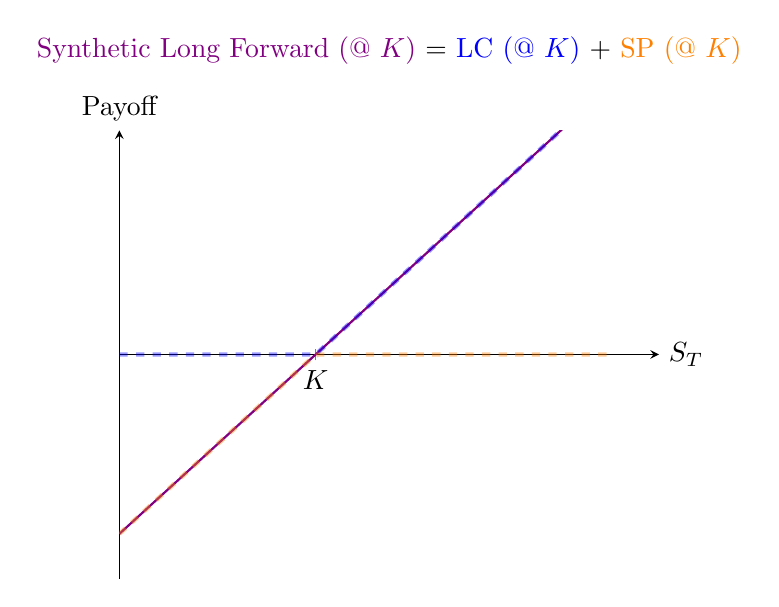
\begin{tikzpicture}[
declare function={
sp(\x) = (\x <= 2) * -(2-\x) + (\x > 2) * 0;
lp(\x) = (\x <= 2) * (2-\x) + (\x > 2) * 0;
sc(\x) = (\x <= 2) * 0 + (\x > 2) * -(\x - 2);
lc(\x) = (\x <= 2) * 0 + (\x > 2) * (\x -2);
}
]
\begin{axis}[domain=0:5, ymin=-2.5, ymax=2.5, xmax=5.5, axis y line=left, axis x line=middle,
title={{\color{violet}Synthetic Long Forward (@ \(K\))} = {\color{blue}LC (@ \(K\))} + {\color{orange}SP (@ \(K\))}},
title style={yshift=0.5cm},
xtick={2}, xticklabels={\(K\)},
ytick=\empty,
ylabel=Payoff,
ylabel style={at={(axis description cs:0,1)}, anchor=south, rotate=-90},
xlabel=\(S_T\),
xlabel style={anchor=west}, samples=75
]
\addplot[violet, thick] {lc(x)+sp(x)};
\addplot[blue, ultra thick, dashed, opacity=0.4] {lc(x)};
\addplot[orange, ultra thick, dashed, opacity=0.4] {sp(x)};
\end{axis}
\end{tikzpicture}

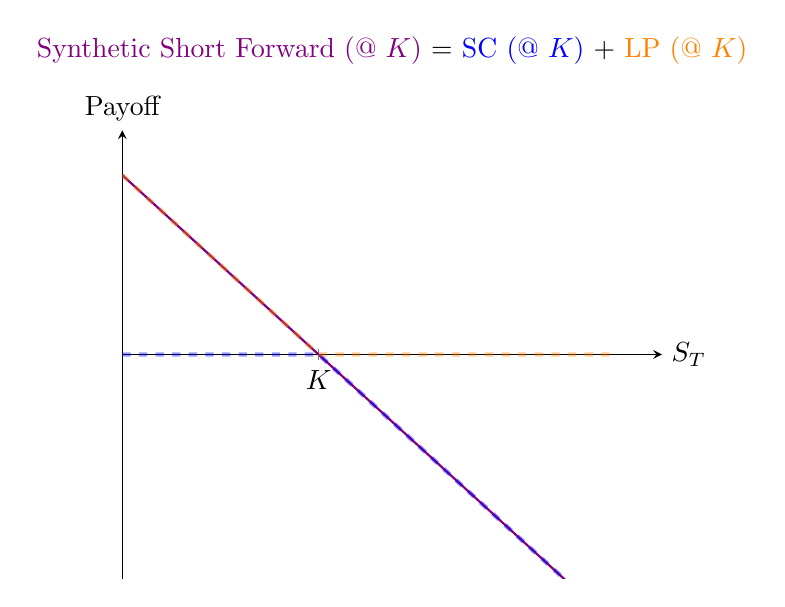
\begin{tikzpicture}[
declare function={
sp(\x) = (\x <= 2) * -(2 - \x) + (\x > 2) * 0;
lp(\x) = (\x <= 2) * (2 - \x) + (\x > 2) * 0;
sc(\x) = (\x <= 2) * 0 + (\x > 2) * -(\x - 2);
lc(\x) = (\x <= 2) * 0 + (\x > 2) * (\x - 2);
}
]
\begin{axis}[domain=0:5, ymin=-2.5, ymax=2.5, xmax=5.5, axis y line=left, axis x line=middle,
title={{\color{violet}Synthetic Short Forward (@ \(K\))} = {\color{blue}SC (@ \(K\))} + {\color{orange}LP (@ \(K\))}},
title style={yshift=0.5cm},
xtick={2}, xticklabels={\(K\)},
ytick=\empty,
ylabel=Payoff,
ylabel style={at={(axis description cs:0,1)}, anchor=south, rotate=-90},
xlabel=\(S_T\),
xlabel style={anchor=west}, samples=75
]
\addplot[violet, thick] {sc(x)+lp(x)};
\addplot[blue, ultra thick, dashed, opacity=0.4] {sc(x)};
\addplot[orange, ultra thick, dashed, opacity=0.4] {lp(x)};
\end{axis}
\end{tikzpicture}
\end{center}

\begin{note}
Algebraically, we can write
\[
\underbrace{(S_T-K)_{+}}_{\text{LC}}+(\underbrace{-(K-S_T)_{+}}_{\text{SP}})
=\begin{cases}
S_T-K+0&\text{if }S_T>K;\\
0-(K-S_T)&\text{if }S_T\le K
\end{cases}
=\underbrace{S_T-K}_{\text{LF}}
\]
and
\[
\underbrace{-(S_T-K)_{+}}_{\text{SC}}+\underbrace{(K-S_T)_{+}}_{\text{LP}}
=\begin{cases}
-(S_T-K)+0&\text{if }S_T>K;\\
0+(K-S_T)&\text{if }S_T\le K
\end{cases}
=\underbrace{K-S_T}_{\text{SF}}.
\]
\end{note}
\item The synthetic long (short) forward has a ``forward price'' of \(K\).  As
we vary the strike price \(K\) for the options, we can compose synthetic
long/short forwards with various ``forward prices'' (unlike the ``genuine''
long/short forward where there is only possible forward price).

\item A main difference between a \emph{synthetic} forward and a \emph{genuine}
forward is that the time-0 value of the latter must be zero (by definition),
while the time-0 value of the former may not be zero. (Prices of call and put
on \faIcon{apple-alt} with the same strike price \(K\) may not be the same.)

\item Let \(C_0(K)\) (\(P_0(K)\)) be the time-0 call (put) price on
\faIcon{apple-alt} (with strike price \(K\)). Then, the time-0 value/price of
the synthetic long forward @ \(K\) is \(C_0(K)-P_0(K)\) (a function of \(K\)).

\item The relationship between call (put) price and its strike price is as follows:
\begin{proposition}
\label{prp:call-put-price-strike-relationship}
The call (put) price \(C_0(K)\) (\(P_0(K)\)) is a strictly decreasing
(increasing) function in \(K\).
\end{proposition}
\begin{pf}
We focus on the call price here, and the proof for the put price is similar.
Assume to the contrary that \(C_0(K')\ge C_0(K)\) for some strike prices
\(K'>K\).  Then, consider the following strategy:
\begin{center}
\begin{tabular}{clr}
\toprule
Time&Transaction&Cash flow\\
\midrule
0&long the call with strike price \(K\)&\(-C_0(K)\)\\
&short the call with strike price \(K'\)&\(+C_0(K')\)\\
&&Total: \(C_0(K')-C_0(K)\ge 0\)\\
\bottomrule
\end{tabular}
\end{center}
Then, the payoff at time \(T\) is given by:
\begin{center}
\begin{tabular}{cccc}
\toprule
Case&LC @ \(K\)&SC @ \(K'\)& Total\\
\midrule
\(S_T\le K\)&\(0\)&\(0\)&\(0\)\\
\(K<S_T\le K'\)&\(S_T-K\)&\(0\)&\(S_T-K>0\)\\
\(S_T>K'\)&\(S_T-K\)&\(S_T-K'\)&\(K'-K>0\)\\
\bottomrule
\end{tabular}
\end{center}
So this is an arbitrage strategy.
\end{pf}

\item Hence, the time-0 price \(C_0(K)-P_0(K)\) is a \emph{strictly decreasing}
function of \(K\). We also know that there is a unique solution \(K^*\) to the
equation
\[
C_0(K)-P_0(K)=0,
\]
namely the no-arbitrage forward price.\footnote{If the solution is not unique,
arbitrage strategy is possible: If there was another solution \(K'>K^*\), then
synthetic short forward @ \(K'\) + ``genuine'' long forward (@ \(K^*\))
\faIcon{arrow-right} zero price + payoff \(K'-K^*>0\) at time \(T\)
\faIcon{arrow-right} arbitrage! Similar for another case.}

So the graph of the function would ``look like'':
\begin{center}
\begin{tikzpicture}[declare function={func(\x) = -0.5+e^(-(\x+0.1)^2);}]
\begin{axis}[domain=0:2, ymin=-0.8, ymax=0.8, axis y line=left, axis x line=middle,
xtick={0.732}, xticklabel={\(K^*\)},
ytick=\empty,
ylabel=Time-0 Price, ylabel style={at={(axis description cs:0,1)}, anchor=south, rotate=-90},
xlabel=\(K\)]
\addplot[blue, thick]{func(x)};
\end{axis}
\end{tikzpicture}
\end{center}
\begin{note}
By the strict decreasingness, we have \(C_0(K)-P_0(K)>0\) for any \(K<K^*\) and
\(C_0(K)-P_0(K)<0\) for any \(K>K^*\). Intuition: We need to pay (receive)
\faIcon{dollar-sign} to long a forward with delivery price less (greater) than
the ``fair'' price \(K^*\).
\end{note}
\end{enumerate}
\subsection{Put-Call Parity}
\label{subsect:put-call-parity}
\begin{enumerate}
\item Recall from \labelcref{it:floor-lc-lb-payoff} that the payoffs of a floor
(long \faIcon{apple-alt} + LP) and ``LC + long bond'' are the same, hence they
have the same (time-0) price. This yields the \emph{put-call parity}:
\begin{theorem}[Put-call parity]
\label{thm:put-call-parity}
We have, under the no-arbitrage principle,
\[
C_0+Ke^{-rT}=S_0+P_0
\]
(for underlying asset \faIcon{apple-alt} with no dividends etc.).
\end{theorem}
\begin{pf}
Note that the price of ``LC + long bond (lending \(Ke^{-rT}\))'' is
\(C_0+Ke^{-rT}\), while the price of the floor (long \faIcon{apple-alt} + LP)
is \(S_0+P_0\).
\end{pf}

This equation relates prices of call and put on \faIcon{apple-alt} with the
same strike price \(K\). (But it does not suggest what their individual prices
are.)

\item The put-call parity can be generalized to be applicable for \emph{any}
underlying asset (which may have dividends):
\begin{theorem}[Generalized put-call parity]
\label{thm:gen-put-call-parity}
Under the no-arbitrage principle,
\[
C_0+Ke^{-rT}=F_0e^{-rT}+P_0
\]
where \(F_0\) is the no-arbitrage forward price (for a forward on \faIcon{apple-alt} negotiated at time 0).  \end{theorem}
\begin{pf}
Recall that a \emph{synthetic long forward} @ \(K\) (LC @ \(K\) + SP @ \(K\))
has the payoff \(S_T-K\), i.e.,
\[
(S_T-K)_{+}-(K-S_T)_{+}=S_T-K.
\]
Rearranging it gives
\[
(S_T-K)_{+}+K=(K-S_T)_{+}+\underbrace{S_T}_{\mathclap{S_T-F_0+F_0}}.
\]
Note that ``LC @ \(K\) + long bond (lending \(Ke^{-rT}\))'' gives the payoff on
LHS, and ``LP @ \(K\) + long forward + long bond (lending \(F_0e^{-rT}\))''
gives the payoff on RHS. By the law of one price, their time-0 values are
equal, i.e.,
\[
\underbrace{C_0+Ke^{-rT}}_{\text{former}}=\underbrace{F_0e^{-rT}+P_0}_{\text{latter}}.
\]
\end{pf}

\begin{note}
When the underlying asset \faIcon{apple-alt} does not have dividends etc., we
have \(F_0=S_0e^{rT}\), and the result reduces to \cref{thm:put-call-parity}.
\end{note}

\item Given a set of call and put prices, if the put-call parity is
\emph{violated}, then it means that there is an arbitrage strategy.

\begin{note}
To obtain such arbitrage strategy, a general idea is to ``buy low and sell
high'' at time 0. For example, if LHS is less than RHS, at time 0, we perform
the transactions ``associated'' with LHS (LC + long bond; ``buy low'') and
perform the \emph{reverse} of the transactions ``associated'' with RHS (short
bond + short forward + SP; ``sell high'').
\end{note}
\end{enumerate}
\subsection{Bull Call/Put Spreads}
\begin{enumerate}
\item An \defn{option spread} consists of long/short options (of the same kind,
i.e., call or put) on the same underlying asset \faIcon{apple-alt}, with the
same expiration date and exercise style, but with different strike prices (the
strike prices are ``spread'' out).

\item Recall the strategies for speculators bullish on \faIcon{apple-alt} in
\labelcref{it:bull-strat}:
\begin{itemize}
\item long \faIcon{apple-alt}
\item long forward on \faIcon{apple-alt}
\item LC on \faIcon{apple-alt}
\item SP on \faIcon{apple-alt}
\end{itemize}
From ``long \faIcon{apple-alt}/long forward on \faIcon{apple-alt}'' to ``LC on
\faIcon{apple-alt}'', the bullish ``extent'' drops. (The profit ``potential''
from the rise \faIcon{chart-line} in price of \faIcon{apple-alt} drops, but the
strategy becomes ``safer''.)
\begin{center}
\begin{tikzpicture}
[declare function={
la(\x) = (x-2);
lc(\x) = (\x <= 2) * -0.5 + (\x > 2) * (x-2.5);
}]
\begin{axis}[domain=0:5, ymin=-2.5, ymax=2.5, xmax=5.5, axis y line=left, axis x line=middle,
xtick=\empty, ytick=\empty, samples=75,
legend entries={Long \faIcon{apple-alt}/Long Forward on \faIcon{apple-alt}, LC},
legend style={legend pos=outer north east},
ylabel=P/L,
ylabel style={at={(axis description cs:0,1)}, anchor=south, rotate=-90},
xlabel=\(S_T\),
xlabel style={anchor=west}
]
\addplot[brown, thick]{la(x)};
\addplot[blue, thick]{lc(x)};
\draw[opacity=0.4, ForestGreen, line width=0.2cm, line cap=round, line join=round] (0,-0.5) -- (2,-0.5)
node[opacity=1, midway, below] {\faIcon{shield-alt}};
\end{axis}
\end{tikzpicture}
\end{center}
To obtain the protection {\color{ForestGreen}\faIcon{shield-alt}} from LC, we
need to pay a call option price \(C_0\) at time 0.

\item A \emph{bull (call) spread} is a strategy to obtain such protection
{\color{ForestGreen}\faIcon{shield-alt}} with a \emph{cheaper} price (at the
expense of the profit ``potential'').

\item Intuitively, the P/L graph of a bull call spread is obtained by
``bending'' a ``later positive'' portion for the P/L graph of LC, in exchange
for a cheaper price:
\begin{center}
\begin{tikzpicture}
[declare function={
sc(\x) = (\x <= 3.5) * 0.2 + (\x > 3.5) * -(x-3.7);
lc(\x) = (\x <= 2) * -0.5 + (\x > 2) * (x-2.5);
}]
\begin{axis}[domain=0:5, ymin=-2.5, ymax=2.5, xmax=5.5, axis y line=left, axis x line=middle,
xtick=\empty, ytick=\empty, samples=75,
ylabel=P/L,
ylabel style={at={(axis description cs:0,1)}, anchor=south, rotate=-90},
xlabel=\(S_T\),
xlabel style={anchor=west}
]
\addplot[violet, thick]{lc(x)+sc(x)};
\addplot[blue, dashed, opacity=0.5, thick]{lc(x)};
\draw[opacity=0.4, ForestGreen, line width=0.2cm, line cap=round, line join=round] (0,-0.3) -- (2,-0.3)
node[opacity=1, midway, above] {\faIcon{shield-alt}};
\draw[-Latex, dashed, brown] (4.3,1.7) to[bend left] (4.5,1.2);
\draw[->, brown] (0.5,-0.5) -- (0.5,-0.3);
\draw[->, brown] (1,-0.5) -- (1,-0.3);
\draw[->, brown] (1.5,-0.5) -- (1.5,-0.3);
\node[brown] () at (2,-0.8) {cheaper};
\node[brown] () at (5,1.7) {``bend''};
\end{axis}
\end{tikzpicture}
\end{center}
\item The ``bending'' is performed by having a SC with a higher strike price
\(K'\) than the strike price for LC (\(K\)), i.e., \defn{bull call spread} is a
combination of LC @ \(K\) and SC @ \(K'\) with \(K'>K\):
\begin{center}
\begin{tikzpicture}
[declare function={
sc(\x) = (\x <= 3.5) * 0.2 + (\x > 3.5) * -(x-3.7);
lc(\x) = (\x <= 2) * -0.5 + (\x > 2) * (x-2.5);
}]
\begin{axis}[domain=0:5, ymin=-2.5, ymax=2.5, xmax=5.5, axis y line=left, axis x line=middle,
xtick={2,3.5}, xticklabels={\(K\),\(K'\)}, xticklabel style={yshift=0.6cm},
ytick=\empty, samples=75,
ylabel=P/L,
ylabel style={at={(axis description cs:0,1)}, anchor=south, rotate=-90},
xlabel=\(S_T\),
xlabel style={anchor=west},
legend entries={LC @ \(K\), SC @ \(K'\)},
legend style={legend pos=outer north east},
title={{\color{violet}\((K,K')\)-Bull Call Spread} = {\color{blue}LC @ \(K\)} + {\color{orange}SC @ \(K'\)}},
title style={yshift=0.5cm}
]
\addplot[blue, dashed, opacity=0.5, thick]{lc(x)};
\addplot[orange, dashed, opacity=0.5, thick]{sc(x)};
\addplot[violet, thick]{lc(x)+sc(x)};
\draw[opacity=0.4, ForestGreen, line width=0.2cm, line cap=round, line join=round] (0,-0.3) -- (2,-0.3)
node[opacity=1, midway, above] {\faIcon{shield-alt}};
\draw[-Latex, dashed, brown] (4.3,1.7) to[bend left] (4.5,1.2);
\draw[->, brown] (0.5,-0.5) -- (0.5,-0.3);
\draw[->, brown] (1,-0.5) -- (1,-0.3);
\draw[->, brown] (1.5,-0.5) -- (1.5,-0.3);
\node[brown] () at (2,-0.8) {cheaper};
\node[brown] () at (5,1.7) {``bend''};
\end{axis}
\end{tikzpicture}
\end{center}
Let \(C_0(K)\) and \(C_0(K')\) be the prices of the call options with the
strike prices \(K\) and \(K'\) respectively. Then, the price of the bull call
spread is \(C_0(K)-C_0(K')\) (which is positive by
\cref{prp:call-put-price-strike-relationship}) \faIcon{arrow-right} cheaper
than LC @ \(K\).
\item The P/L of the bull call spread is
\[
(S_T-K)_{+}-(S_T-K')_{+}-(C_0(K)-C_0(K'))e^{rT}.
\]
\item It turns out that we can obtain the same P/L graph using \emph{put}
options instead, and the strategy is known as \defn{bull put spread} (LP @
\(K\) + SP @ \(K'\)). First we consider its \emph{payoff} graph:
\begin{center}
\begin{tikzpicture}
[declare function={
sp(\x) = (\x <= 3.5) * -(3.5-x) + (\x > 3.5) * 0;
lp(\x) = (\x <= 2) * (2-x) + (\x > 2) * 0;
}]
\begin{axis}[domain=0:5, ymin=-2.5, ymax=2.5, xmax=5.5, axis y line=left, axis x line=middle,
xtick={2,3.5}, xticklabels={\(K\),\(K'\)}, xticklabel style={yshift=0.6cm},
ytick=\empty, samples=75,
ylabel=Payoff,
ylabel style={at={(axis description cs:0,1)}, anchor=south, rotate=-90},
xlabel=\(S_T\),
xlabel style={anchor=west},
legend entries={LP @ \(K\), SP @ \(K'\)},
legend style={legend pos=outer north east},
title={{\color{violet}Bull Put Spread} = {\color{blue}LP @ \(K\)} + {\color{orange}SP @ \(K'\)}},
title style={yshift=0.5cm}
]
\addplot[blue, dashed, opacity=0.5, thick]{lp(x)};
\addplot[orange, dashed, opacity=0.5, thick]{sp(x)};
\addplot[violet, thick]{lp(x)+sp(x)};
\end{axis}
\end{tikzpicture}
\end{center}
\begin{note}
The ``shape'' of this graph is the same as the one for the P/L graph of bull
call spread.
\end{note}

\item Let \(P_0(K)\) and \(P_0(K')\) be the prices of the put options with the
strike prices \(K\) and \(K'\) respectively.  The time-0 value of the bull put
spread is \(P_0(K)-P_0(K')\), which is \emph{negative} by
\cref{prp:call-put-price-strike-relationship}.

Now, since the P/L of the bull put spread is
\[
(K-S_T)_{+}-(K'-S_T)_{+}-(P_0(K)-P_0(K'))e^{rT},
\]
its P/L graph is obtained by from shifting \emph{upward} the payoff graph.

\item The P/L graph obtained here \emph{must} coincide with the P/L graph for
bull call spread, or else there would be an arbitrage opportunity (short
``spread with `higher' P/L graph'' and long ``spread with `lower' P/L
graph'' \faIcon{arrow-right} ``net'' P/L is a positive constant
\emph{always} \faIcon{arrow-right} arbitrage!\footnote{When P/L is always
positive, it means the resulting cash flow at time \(T\) after accumulating all
past cash flows to that time is \emph{positive} \faIcon{arrow-right} possible
to have no cash outflow but have a positive cash flow at time \(T\)
\faIcon{arrow-right} arbitrage!}):
\begin{center}
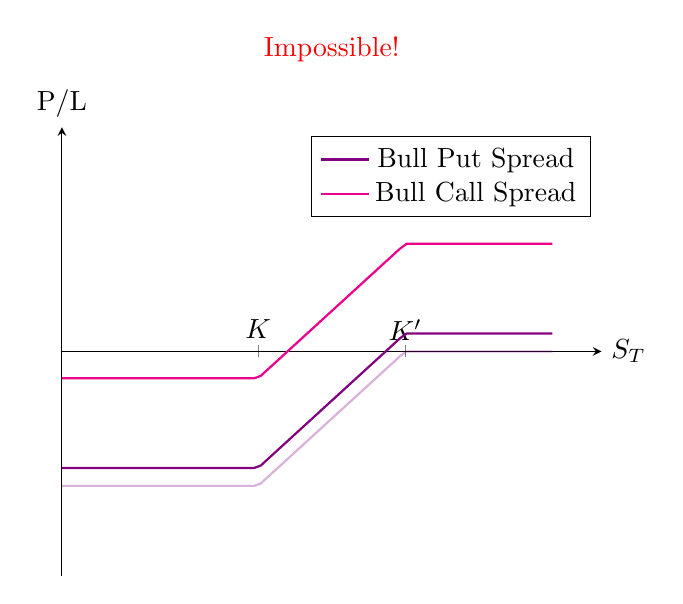
\begin{tikzpicture}
[declare function={
sp(\x) = (\x <= 3.5) * -(3.5-x) + (\x > 3.5) * 0;
lp(\x) = (\x <= 2) * (2-x) + (\x > 2) * 0;
}]
\begin{axis}[domain=0:5, ymin=-2.5, ymax=2.5, xmax=5.5, axis y line=left, axis x line=middle,
xtick={2,3.5}, xticklabels={\(K\),\(K'\)}, xticklabel style={yshift=0.6cm},
ytick=\empty, samples=75,
ylabel=P/L,
ylabel style={at={(axis description cs:0,1)}, anchor=south, rotate=-90},
xlabel=\(S_T\),
xlabel style={anchor=west},
title={\color{red}Impossible!},
title style={yshift=0.5cm},
legend entries={,Bull Put Spread,Bull Call Spread},
]
\addplot[violet, thick, opacity=0.3]{lp(x)+sp(x)};
\addplot[violet, thick]{lp(x)+sp(x)+0.2};
\addplot[magenta, thick]{lp(x)+sp(x)+1.2};
\end{axis}
\end{tikzpicture}

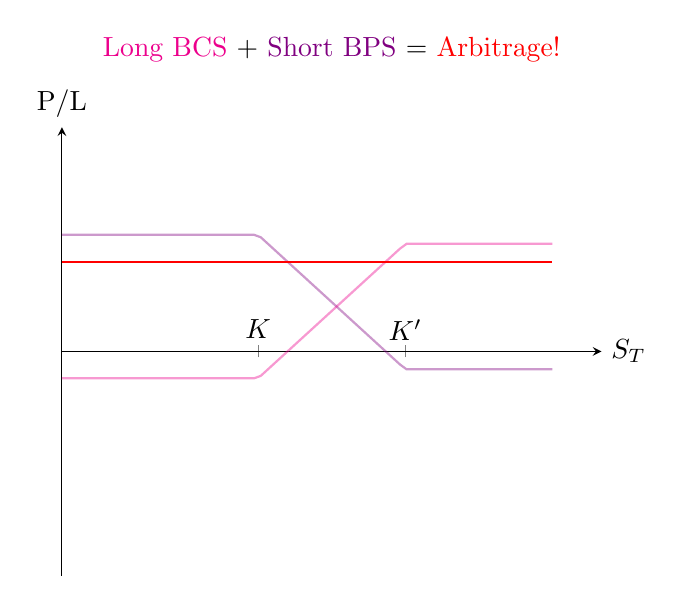
\begin{tikzpicture}
[declare function={
sp(\x) = (\x <= 3.5) * -(3.5-x) + (\x > 3.5) * 0;
lp(\x) = (\x <= 2) * (2-x) + (\x > 2) * 0;
}]
\begin{axis}[domain=0:5, ymin=-2.5, ymax=2.5, xmax=5.5, axis y line=left, axis x line=middle,
xtick={2,3.5}, xticklabels={\(K\),\(K'\)}, xticklabel style={yshift=0.6cm},
ytick=\empty, samples=75,
ylabel=P/L,
ylabel style={at={(axis description cs:0,1)}, anchor=south, rotate=-90},
xlabel=\(S_T\),
xlabel style={anchor=west},
title={{\color{magenta}Long BCS} + {\color{violet}Short BPS} = {\color{red}Arbitrage!}},
title style={yshift=0.5cm},
]
%\addplot[violet, thick, opacity=0.3]{lp(x)+sp(x)};
\addplot[violet, thick, opacity=0.4]{-(lp(x)+sp(x)+0.2)};
\addplot[magenta, thick, opacity=0.4]{lp(x)+sp(x)+1.2};
\addplot[red, thick]{1};
\end{axis}
\end{tikzpicture}
\end{center}
The proper P/L graph of bull put spread should coincide with the one for bull
call spread:
\begin{center}
\begin{tikzpicture}
[declare function={
sp(\x) = (\x <= 3.5) * -(3.5-x) + (\x > 3.5) * 0;
lp(\x) = (\x <= 2) * (2-x) + (\x > 2) * 0;
lc(\x) = (\x <= 2) * -0.5 + (\x > 2) * (x-2.5);
}]
\begin{axis}[domain=0:5, ymin=-2.5, ymax=2.5, xmax=5.5, axis y line=left, axis x line=middle,
xtick={2,3.5}, xticklabels={\(K\),\(K'\)}, xticklabel style={yshift=0.6cm},
ytick=\empty, samples=75,
xlabel=\(S_T\),
xlabel style={anchor=west},
title={\color{violet}Bull Call/Put Spread},
title style={yshift=0.5cm},
legend entries={Bull Call/Put Spread (P/L),LC @ \(K\) (P/L), Bull Put Spread (Payoff)},
legend style={legend pos=outer north east},
]
\addplot[violet, thick]{lp(x)+sp(x)+1.2};
\addplot[blue, dashed, opacity=0.5, thick]{lc(x)};
\addplot[violet, thick, opacity=0.3]{lp(x)+sp(x)};
\draw[-Latex, magenta] (0.5,-1.4) -- (0.5,-0.6);
\draw[-Latex, magenta] (1.5,-1.4) -- (1.5,-0.6);
\draw[-Latex, magenta] (2.7,-0.7) -- (2.7,0.3);
\draw[-Latex, magenta] (3.8,0.1) -- (3.8,1.1);
\draw[-Latex, magenta] (4.5,0.1) -- (4.5,1.1);
\draw[opacity=0.4, ForestGreen, line width=0.2cm, line cap=round, line join=round] (0,-0.3) -- (2,-0.3)
node[opacity=1, midway, above] {\faIcon{shield-alt}};
\draw[-Latex, dashed, brown] (4.3,1.7) to[bend left] (4.5,1.2);
\draw[->, brown] (0.5,-0.5) -- (0.5,-0.3);
\draw[->, brown] (1,-0.5) -- (1,-0.3);
\draw[->, brown] (1.5,-0.5) -- (1.5,-0.3);
\end{axis}
\end{tikzpicture}
\end{center}
\begin{note}
Since bull call spread and bull put spread have identical P/L, they are not
that much ``different''. Thus, sometimes we just use the term \defn{bull
spread} to refer to either of them.
\end{note}
\end{enumerate}
\subsection{Bear Call/Put Spreads}
\begin{enumerate}
\item \emph{Bear call/put spread} is simply \emph{reverse} bull call/put
spread, as one may expect.

\begin{intuition}
The \emph{reverse} of a strategy for \emph{bullish} speculators should be for
\emph{bearish} speculators.
\end{intuition}

\item More precisely, we have:
\begin{itemize}
\item \defn{bear call spread} = SC @ \(K\) + LC @ \(K'\)
\item \defn{bear put spread} = SP @ \(K\) + LP @ \(K'\)
\end{itemize}

\item The payoff (P/L) of a bear call/put spread is simply the negative of the
payoff (P/L) of the respective bull call/put spread. Hence, we again sometimes
just use the term \defn{bear spread} to refer to either of them.
\begin{note}
The payoff (P/L) graph of a bear spread is just the mirror image of the payoff
(P/L) graph of the respective bull spread along the \(S_T\)-axis.
\end{note}
\end{enumerate}
\subsection{Box Spreads}
\begin{enumerate}
\item A \emph{box spread} \faIcon{box} is a ``synthetic (risk-free) bond''
created using options, i.e., its payoff (at time \(T\)) is a positive constant
always (and its price is \(\text{payoff}\times e^{-rT}\)).
\item To get such a constant payoff, synthetic forwards are utilized:
\begin{center}
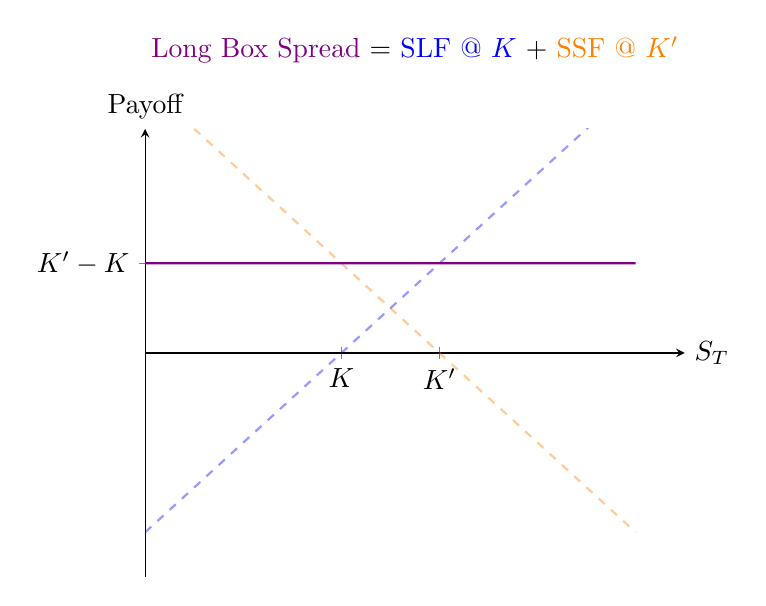
\begin{tikzpicture}[
declare function={
sp(\x) = (\x <= 2) * -(2 - \x) + (\x > 2) * 0;
lc(\x) = (\x <= 2) * 0 + (\x > 2) * (\x - 2);
sc(\x) = (\x <= 3) * 0 + (\x > 3) * -(\x - 3);
lp(\x) = (\x <= 3) * (3 - \x) + (\x > 3) * 0;
}
]
\begin{axis}[domain=0:5, ymin=-2.5, ymax=2.5, xmax=5.5, axis y line=left, axis x line=middle,
title={{\color{violet}Long Box Spread} = {\color{blue}SLF @ \(K\)} + {\color{orange}SSF @ \(K'\)}},
title style={yshift=0.5cm}, xtick={2,3}, xticklabels={\(K\), \(K'\)},
ytick={1}, yticklabels={\(K'-K\)},
ylabel=Payoff,
ylabel style={at={(axis description cs:0,1)}, anchor=south, rotate=-90},
xlabel=\(S_T\),
xlabel style={anchor=west}, samples=75
]
\addplot[orange, dashed, thick, opacity=0.4] {sc(x)+lp(x)};
\addplot[blue, dashed, thick, opacity=0.4] {sp(x)+lc(x)};
\addplot[violet, thick] {sc(x)+lp(x)+sp(x)+lc(x)};
\end{axis}
\end{tikzpicture}
\end{center}

\item A \defn{long box spread} (long position in box spread \faIcon{box}) comprises
of a synthetic long forward @ \(K\) and a synthetic short forward @ \(K'\),
where \(K'>K\). (It mimics a long position in a risk-free bond.) A \defn{short
box spread} is a short position in box spread \faIcon{box}: It also consists of
a synthetic long forward @ \(K\) and a synthetic short forward @ \(K'\), but
\(K'<K\):
\begin{center}
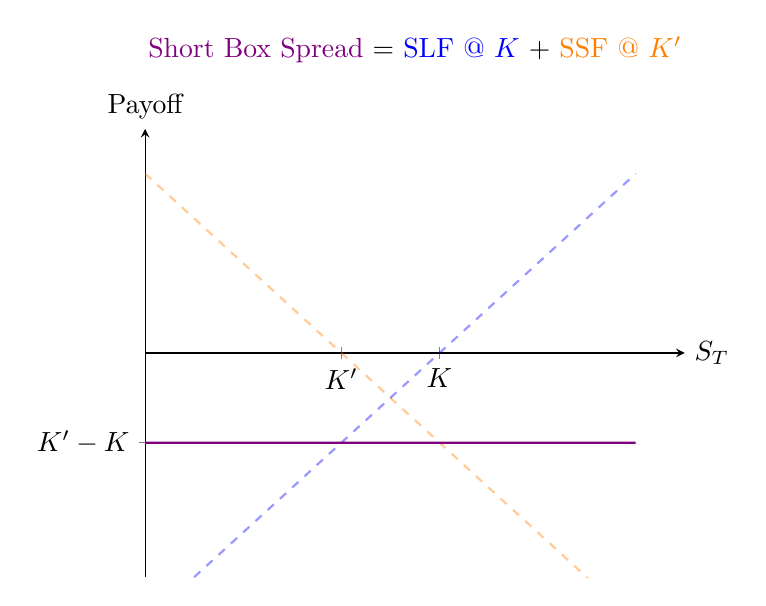
\begin{tikzpicture}[
declare function={
sp(\x) = (\x <= 3) * -(3 - \x) + (\x > 3) * 0;
lc(\x) = (\x <= 3) * 0 + (\x > 3) * (\x - 3);
sc(\x) = (\x <= 2) * 0 + (\x > 2) * -(\x - 2);
lp(\x) = (\x <= 2) * (2 - \x) + (\x > 2) * 0;
}
]
\begin{axis}[domain=0:5, ymin=-2.5, ymax=2.5, xmax=5.5, axis y line=left, axis x line=middle,
title={{\color{violet}Short Box Spread} = {\color{blue}SLF @ \(K\)} + {\color{orange}SSF @ \(K'\)}},
title style={yshift=0.5cm},
xtick={2,3}, xticklabels={\(K'\), \(K\)},
ytick={-1}, yticklabels={\(K'-K\)},
ylabel=Payoff,
ylabel style={at={(axis description cs:0,1)}, anchor=south, rotate=-90},
xlabel=\(S_T\),
xlabel style={anchor=west}, samples=75
]
\addplot[orange, dashed, thick, opacity=0.4] {sc(x)+lp(x)};
\addplot[blue, dashed, thick, opacity=0.4] {sp(x)+lc(x)};
\addplot[violet, thick] {sc(x)+lp(x)+sp(x)+lc(x)};
\end{axis}
\end{tikzpicture}
\end{center}

\item The payoff of a long/short box spread (at time \(T\)) is \(K'-K\). Hence,
its time-0 value is \((K'-K)e^{-rT}\) \faIcon{arrow-right} its P/L is simply
zero always.

\item To be more explicit about the option positions used in a long/short box
spread, we can write:
\[
\text{long/short box spread}
= \text{SLF @ \(K\)} + \text{SSF @ \(K'\)} 
= \text{LC @ \(K\)} + \text{SP @ \(K\)} + \text{LP @ \(K'\)} + \text{SC @ \(K'\)}.
\]
We can collect the option positions used in the form of a table (or
\emph{box}):
\begin{center}
\begin{tabular}{ccc}
\toprule
Strike Price&Call&Put\\
\midrule
\(K\)&Long&Short\\
\(K'\)&Short&Long\\
\bottomrule
\end{tabular}
\end{center}
Reading it \emph{horizontally} suggests the construction of box spread using
\emph{synthetic forwards}. Reading it \emph{vertically} suggests another way of
composing a long box spread using bull and bear spreads: bull call spread
@ \((K,K')\) + bear put spread @ \((K,K')\).

\begin{center}
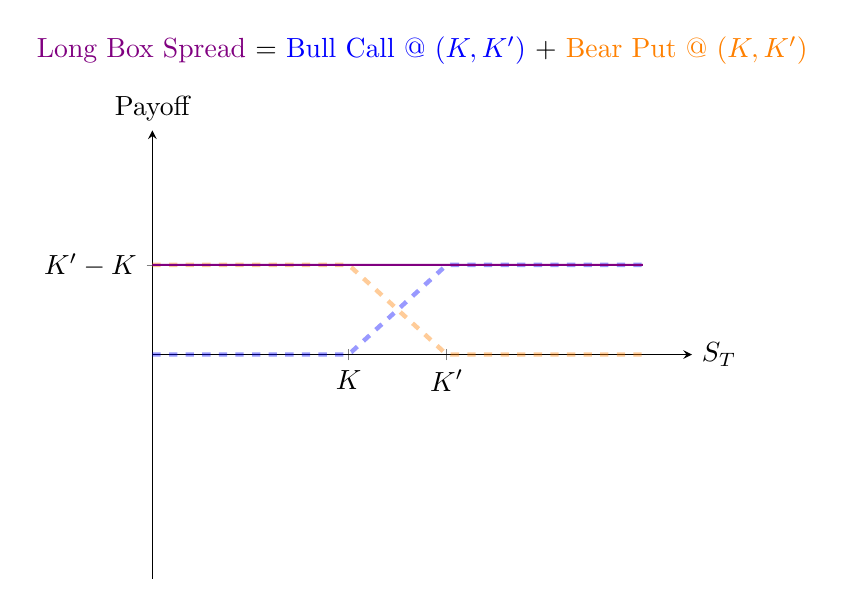
\begin{tikzpicture}[
declare function={
sp(\x) = (\x <= 2) * -(2 - \x) + (\x > 2) * 0;
lc(\x) = (\x <= 2) * 0 + (\x > 2) * (\x - 2);
sc(\x) = (\x <= 3) * 0 + (\x > 3) * -(\x - 3);
lp(\x) = (\x <= 3) * (3 - \x) + (\x > 3) * 0;
}
]
\begin{axis}[domain=0:5, ymin=-2.5, ymax=2.5, xmax=5.5, axis y line=left, axis x line=middle,
title={{\color{violet}Long Box Spread} = {\color{blue}Bull Call @ \((K,K')\)} + {\color{orange}Bear Put @ \((K,K')\)}},
title style={yshift=0.5cm}, xtick={2,3}, xticklabels={\(K\), \(K'\)},
ytick={1}, yticklabels={\(K'-K\)},
ylabel=Payoff,
ylabel style={at={(axis description cs:0,1)}, anchor=south, rotate=-90},
xlabel=\(S_T\),
xlabel style={anchor=west}, samples=75
]
\addplot[blue, dashed, ultra thick, opacity=0.4] {sc(x)+lc(x)};
\addplot[orange, dashed, ultra thick, opacity=0.4] {sp(x)+lp(x)};
\addplot[violet, thick] {sc(x)+lp(x)+sp(x)+lc(x)};
\end{axis}
\end{tikzpicture}
\end{center}
\end{enumerate}
\subsection{Ratio Spreads}
\begin{enumerate}
\item A \defn{ratio spread} consists of longing \(m\) calls/puts with one
strike price \(K\) and shorting \(n\) calls/puts (resp.) with another strike
price \(K'\ne K\), where \(m \ne n\).

\begin{remark}
\item A ratio spread is similar to bull/bear call/put spread, except that the
number of calls/puts longed is different from the number of calls/puts shorted.
\item \(m:n\) is the ``ratio'' for the ratio spread.
\end{remark}

\item A ratio spread is a very ``flexible'' strategy and it can have many
different payoff patterns, depending on the ratio and the option type
(call/put). Some examples of payoff graphs:
\begin{center}
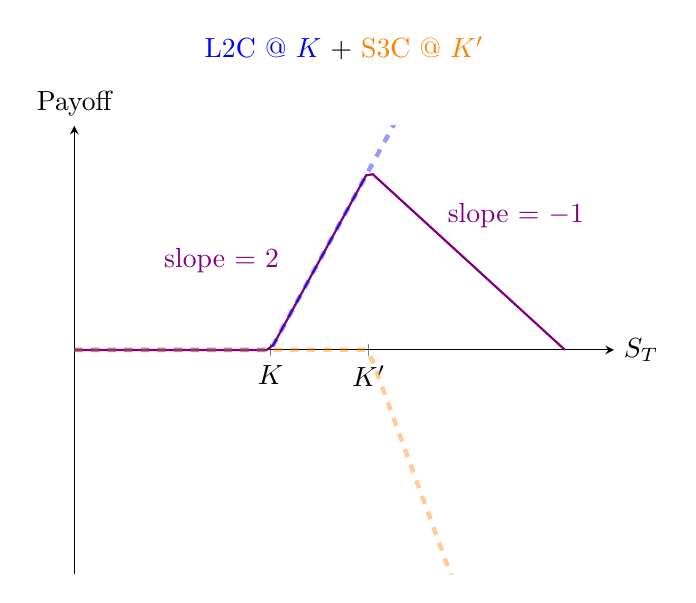
\begin{tikzpicture}[
declare function={
sp(\x) = (\x <= 2) * -(2 - \x) + (\x > 2) * 0;
lc(\x) = (\x <= 2) * 0 + (\x > 2) * (\x - 2);
sc(\x) = (\x <= 3) * 0 + (\x > 3) * -(\x - 3);
lp(\x) = (\x <= 3) * (3 - \x) + (\x > 3) * 0;
}
]
\begin{axis}[domain=0:5, ymin=-2.5, ymax=2.5, xmax=5.5, axis y line=left, axis x line=middle,
title={{\color{blue}L2C @ \(K\)} + {\color{orange} S3C @ \(K'\)}},
title style={yshift=0.5cm}, xtick={2,3}, xticklabels={\(K\), \(K'\)},
ytick=\empty,
ylabel=Payoff,
ylabel style={at={(axis description cs:0,1)}, anchor=south, rotate=-90},
xlabel=\(S_T\),
xlabel style={anchor=west}, samples=75,
]
\addplot[violet, thick] {2*lc(x)+3*sc(x)};
\addplot[blue, dashed, ultra thick, opacity=0.4] {2*lc(x)};
\addplot[orange, dashed, ultra thick, opacity=0.4] {3*sc(x)};
\node[violet] () at (1.5,1) {slope = 2};
\node[violet] () at (4.5,1.5) {slope = \(-1\)};
\end{axis}
\end{tikzpicture}

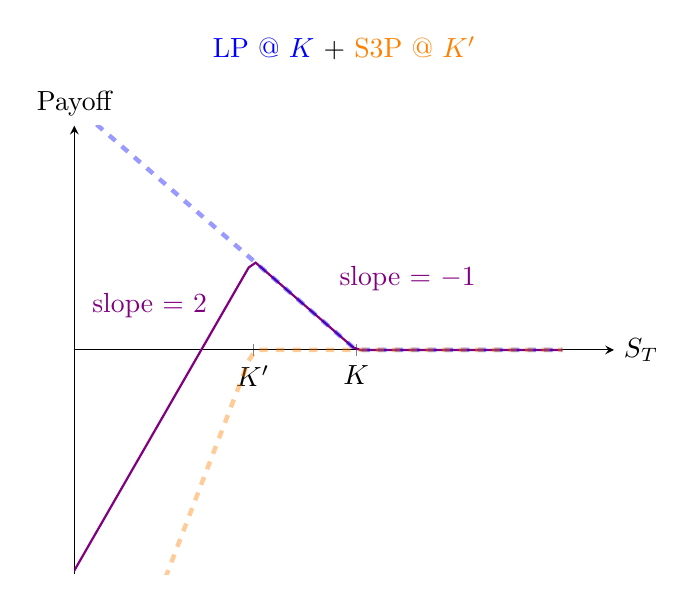
\begin{tikzpicture}[
declare function={
lc(\x) = (\x <= 3) * 0 + (\x > 3) * (\x - 3);
sc(\x) = (\x <= 2) * 0 + (\x > 2) * -(\x - 2);
sp(\x) = (\x <= 2) * -(2 - \x) + (\x > 2) * 0;
lp(\x) = (\x <= 3) * (3 - \x) + (\x > 2) * 0;
}
]
\begin{axis}[domain=0:5, ymin=-2.5, ymax=2.5, xmax=5.5, axis y line=left, axis x line=middle,
title={{\color{blue}LP @ \(K\)} + {\color{orange} S3P @ \(K'\)}},
title style={yshift=0.5cm}, xtick={2,3}, xticklabels={\(K'\), \(K\)},
ytick=\empty,
ylabel=Payoff,
ylabel style={at={(axis description cs:0,1)}, anchor=south, rotate=-90},
xlabel=\(S_T\),
xlabel style={anchor=west}, samples=75,
]
\addplot[violet, thick] {1*lp(x)+3*sp(x)};
\addplot[blue, dashed, ultra thick, opacity=0.4] {lp(x)};
\addplot[orange, dashed, ultra thick, opacity=0.4] {3*sp(x)};
\node[violet] () at (1,0.5) {slope = 2};
\node[violet] () at (3.5,0.8) {slope = \(-1\)};
\end{axis}
\end{tikzpicture}
\end{center}
\end{enumerate}
\subsection{Collars}
\begin{enumerate}
\item A \defn{collar} consists of LP @ \(K\) + SC @ \(K'\) with \(K'>K\) (both
options are on the same asset and have the same expiration date):
\begin{center}
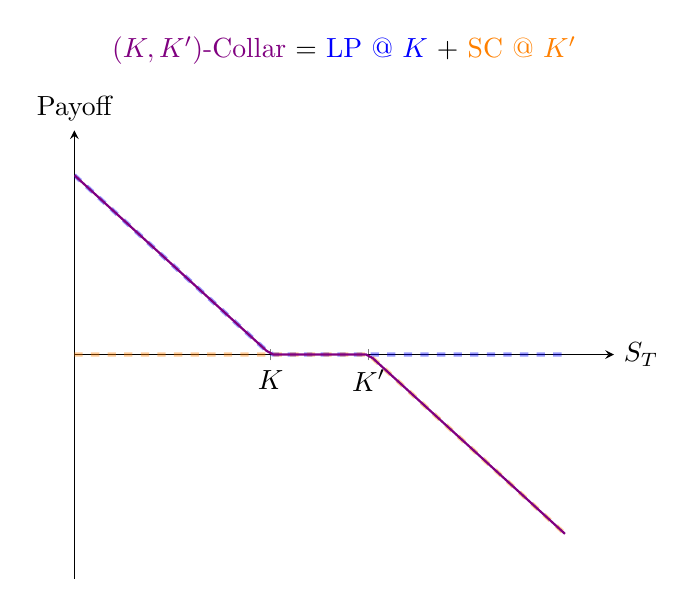
\begin{tikzpicture}[
declare function={
lc(\x) = (\x <= 3) * 0 + (\x > 3) * (\x - 3);
lp(\x) = (\x <= 2) * (2 - \x) + (\x > 2) * 0;
sp(\x) = (\x <= 2) * -(2 - \x) + (\x > 2) * 0;
sc(\x) = (\x <= 3) * 0 + (\x > 3) * -(\x - 3);
}
]
\begin{axis}[domain=0:5, ymin=-2.5, ymax=2.5, xmax=5.5, axis y line=left, axis x line=middle,
title={{\color{violet}\((K, K')\)-Collar} = {\color{blue}LP @ \(K\)} + {\color{orange}SC @ \(K'\)}},
title style={yshift=0.5cm}, xtick={2,3}, xticklabels={\(K\), \(K'\)},
ytick=\empty,
ylabel={Payoff},
ylabel style={at={(axis description cs:0,1)}, anchor=south, rotate=-90},
xlabel={\(S_T\)},
xlabel style={anchor=west}, samples=75
]
\addplot[blue, dashed, ultra thick, opacity=0.4] {lp(x)};
\addplot[orange, dashed, ultra thick, opacity=0.4] {sc(x)};
\addplot[violet, thick] {lp(x)+sc(x)};
\end{axis}
\end{tikzpicture}
\end{center}

\item The main usage of collar is to insure a long position in
\faIcon{apple-alt}.  Recall that a \emph{floor} is a way to hedge such risk (by
adding LP on top of long \faIcon{apple-alt}). The ``initial positive'' part of
payoff (P/L) of LP helps reducing the risk:

\begin{center}
\begin{tikzpicture}[
declare function={
lp(\x) = (\x <= 2) * (1.5-\x) + (\x > 2) * (-0.5);
la(\x) = (\x-2.2);
}
]
\begin{axis}[domain=0:5, ymin=-2.5, ymax=2.5, xmax=5.5, axis y line=left, axis x line=middle,
title={{\color{violet}Floor} = {\color{blue}Long \faIcon{apple-alt}} + {\color{orange}LP @ \(K\)}},
xtick={2}, xticklabel={\(K\)}, xticklabel style={yshift=0.7cm, xshift=0.2cm},
ytick={-2.2},
yticklabel={\(-S_0e^{rT}\)},
ylabel={P/L},
ylabel style={at={(axis description cs:0,1)}, anchor=south, rotate=-90},
xlabel={\(S_T\)},
xlabel style={anchor=west}, samples=75
]
\addplot[blue, thick, dashed, opacity=0.5]{la(x)};
\addplot[orange, thick, dashed, opacity=0.5]{lp(x)};
\addplot[violet, thick]{la(x)+lp(x)};
\draw[opacity=0.4, ForestGreen, line width=0.2cm, line cap=round, line join=round] (0,-0.7) -- (2,-0.7) -- (2.6,-0.1);
\node[ForestGreen] at (1.2,-0.4) {hedged \faIcon{shield-alt} risk};
\end{axis}
\end{tikzpicture}
\end{center}


\item However, for the floor, we need to pay the put option price \(P_0(K)\).
To reduce the initial expense, a \emph{collar} can be used instead of LP.
(Note that the payoff graph of collar also has an ``initial positive'' part.)

\begin{note}
We call ``long \faIcon{apple-alt} + collar'' as \defn{collared}
\faIcon{apple-alt}.  (We usually use this terminology for \emph{stock}:
collared stock.)
\end{note}

Since the time-0 value of a collar is \(P_0(K)-C_0(K')\), which is less than
\(P_0(K)\), this insurance is ``cheaper''. Of course there is no ``free lunch''
and the thing we give up is the profit ``potential'':
\begin{center}
\begin{tikzpicture}[
declare function={
lp(\x) = (\x <= 2) * (1.5-x) + (\x > 2) * -0.5;
sc(\x) = (\x <= 3) * 0.3 + (\x > 3) * -(x-3.3);
la(\x) = (\x-2.2);
}
]
\begin{axis}[
domain=0:5, ymin=-2.5, ymax=2.5, xmax=5.5, axis y line=left, axis x line=middle,
title={{\color{violet}Collared \faIcon{apple-alt}} = {\color{blue}Long \faIcon{apple-alt}} + {\color{orange}\((K, K')\)-Collar}},
title style={yshift=0.5cm},
xtick={2,3}, xticklabels={\(K\),\(K'\)}, xticklabel style={yshift=0.7cm, xshift=0.2cm},
ytick={-2.2},
yticklabel={\(-S_0e^{rT}\)},
ylabel={P/L},
ylabel style={at={(axis description cs:0,1)}, anchor=south, rotate=-90},
xlabel={\(S_T\)},
xlabel style={anchor=west}, samples=75,
legend entries={Collared \faIcon{apple-alt}, Floor},
legend style={legend pos=outer north east}
]
\addplot[violet, thick]{la(x) + lp(x) + sc(x)};
\addplot[opacity=0.4, magenta, thick]{la(x)+lp(x)};
\addplot[blue, thick, dashed, opacity=0.5]{la(x)};
\addplot[orange, thick, dashed, opacity=0.5]{lp(x) + sc(x)};
\draw[opacity=0.4, ForestGreen, line width=0.2cm, line cap=round, line join=round] (0,-0.4) -- (2,-0.4) -- (2.3,-0.1);
\end{axis}
\end{tikzpicture}
\end{center}
After taking a collar, the range of P/L gets restricted to a ``narrow''
range, just like a physical \emph{collar} put around the neck of an animal that
restricts its ``movement''. By varying \(K\) and \(K'\) (such that \(K'>K\) of
course), we can ``place'' the restriction at different ``locations'' and
control its ``strength'' (how ``narrow'').

\item The time-0 value of a collar \(P_0(K)-C_0(K')\) can be positive,
negative, or zero (depending on the choice of \(K\) and \(K'\)). If it is zero,
the collar is called \defn{zero-cost collar}.

\begin{intuition}
For zero-cost collar, the ``protection'' sources completely from the profit
potential given up, since we do not pay any money for this insurance.
\end{intuition}

\item However, if the strike price \(K\) specified is ``too high'', then it is
impossible to construct a zero-cost collar, as suggested by the following
result:
\begin{proposition}
\label{prp:k-high-collar-val-positive}
If \(K\ge S_0e^{rT}\) (the no-arbitrage forward price), then for any \(K'>K\),
\[
C_0(K')<P_0(K)
\]
(so the time-0 value of the collar is always positive).
\end{proposition}
\begin{pf}
For any \(K'>K\),
\begin{align*}
P_0(K)&=C_0(K)+Ke^{-rT}-S_0&\text{(put-call parity)}\\
&>C_0(K')+{\color{violet}K}e^{-rT}-S_0&\text{(\cref{prp:call-put-price-strike-relationship})}\\
&\ge C_0(K')+{\color{violet}S_0e^{rT}}e^{-rT}-S_0\\
&=C_0(K').
\end{align*}
\end{pf}
\end{enumerate}
\subsection{Straddles}
\label{subsect:straddles}
\begin{enumerate}
\item Sometimes speculators are \emph{neither bullish nor bearish}, and
they speculate the \emph{volatility} instead. They are not speculating the
\emph{direction} of future price movement, but its \emph{magnitude} (large
movement \faIcon{arrow-right} high ``volatility''; small movement
\faIcon{arrow-right} low ``volatility'').
\item Some option strategies for volatility speculation are discussed in
\cref{subsect:straddles,subsect:strangles,subsect:butterfly-sprd}.
\item A \defn{straddle} is a combination of call and put on the same asset
\faIcon{apple-alt}, with the same strike price and expiration date.

\item The payoff graph of straddle:
\begin{center}
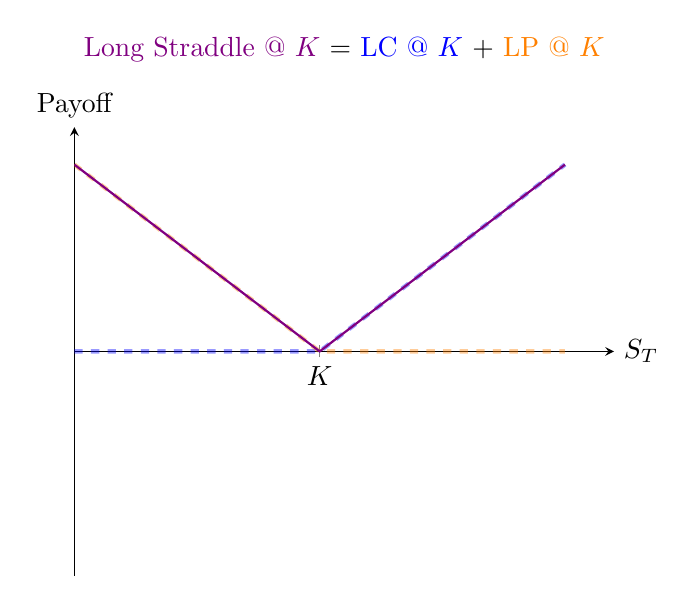
\begin{tikzpicture}[
declare function={
lc(\x) = (\x <= 2.5) * 0 + (\x > 2.5) * (\x - 2.5);
lp(\x) = (\x <= 2.5) * (2.5 - \x) + (\x > 2.5) * 0;
}
]
\begin{axis}[domain=0:5, ymin=-3, ymax=3, xmax=5.5, axis y line=left, axis x line=middle,
title={{\color{violet}Long Straddle @ \(K\)} = {\color{blue}LC @ \(K\)} + {\color{orange}LP @ \(K\)}},
title style={yshift=0.5cm}, xtick={2.5}, xticklabels={\(K\)},
ytick=\empty,
ylabel={Payoff},
ylabel style={at={(axis description cs:0,1)}, anchor=south, rotate=-90},
xlabel={\(S_T\)},
xlabel style={anchor=west}, samples=75
]
\addplot[blue, dashed, ultra thick, opacity=0.4] {lc(x)};
\addplot[orange, dashed, ultra thick, opacity=0.4] {lp(x)};
\addplot[violet, thick] {lc(x)+lp(x)};
\end{axis}
\end{tikzpicture}
\end{center}
\begin{note}
The ``shape'' of the graph looks like the act of ``straddling'' (sitting
astride), from ``top view''.
\end{note}


\item The time-0 price of a straddle is \(C_0+P_0\), which is positive. Hence,
its P/L graph can be obtained by shifting its payoff graph downward:
\begin{center}
\begin{tikzpicture}[
declare function={
lc(\x) = (\x <= 2.5) * 0 + (\x > 2.5) * (\x - 2.5);
lp(\x) = (\x <= 2.5) * (2.5 - \x) + (\x > 2.5) * 0;
}
]
\begin{axis}[domain=0:5, ymin=-3, ymax=3, xmax=5.5, axis y line=left, axis x line=middle,
title={{\color{violet}Long Straddle}},
title style={yshift=0.5cm}, xtick={2.5}, xticklabels={\(K\)},
ytick={-0.8}, yticklabels={\(-(C_0+P_0)e^{rT}\)},
ylabel={P/L},
ylabel style={at={(axis description cs:0,1)}, anchor=south, rotate=-90},
xlabel={\(S_T\)},
xlabel style={anchor=west}, samples=75
]
\addplot[violet, opacity=0.4, thick] {lc(x)+lp(x)};
\addplot[violet, thick] {lc(x)+lp(x)-0.8};
\draw[-Latex, brown] (1,1.3) -- (1,0.8);
\draw[-Latex, brown] (1.5,0.8) -- (1.5,0.3);
\draw[-Latex, brown] (3.5,0.8) -- (3.5,0.3);
\draw[-Latex, brown] (4,1.3) -- (4,0.8);
\end{axis}
\end{tikzpicture}
\end{center}

\item To speculate \emph{high} volatility (large future price movement in
either direction), one can long straddle.

\item On the other hand, if one want to speculate \emph{low} volatility (small
future price movement in either direction), one can \emph{short} straddle (SC @
\(K\) + SP @ \(K\)).

\item The payoff and P/L graphs of short straddle:
\begin{center}
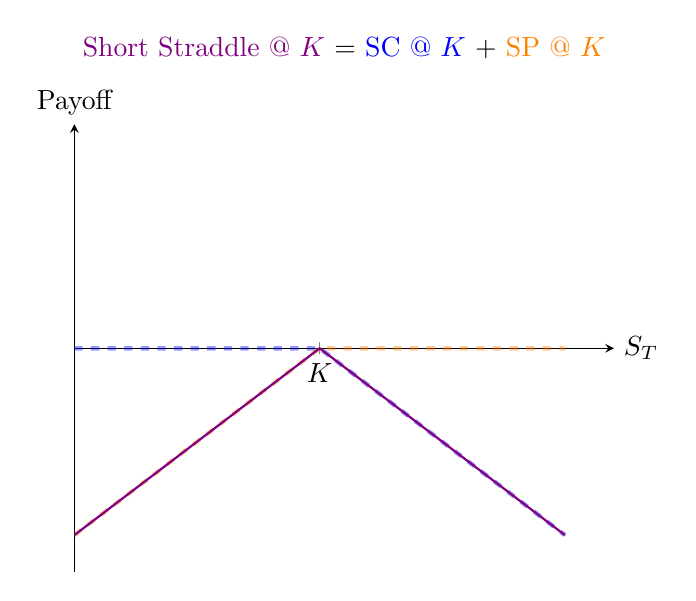
\begin{tikzpicture}[
declare function={
lc(\x) = (\x <= 2.5) * 0 + (\x > 2.5) * (\x - 2.5);
lp(\x) = (\x <= 2.5) * (2.5 - \x) + (\x > 2.5) * 0;
}
]
\begin{axis}[domain=0:5, ymin=-3, ymax=3, xmax=5.5, axis y line=left, axis x line=middle,
title={{\color{violet}Short Straddle @ \(K\)} = {\color{blue}SC @ \(K\)} + {\color{orange}SP @ \(K\)}},
title style={yshift=0.5cm}, xtick={2.5}, xticklabels={\(K\)},
ytick=\empty,
ylabel={Payoff},
ylabel style={at={(axis description cs:0,1)}, anchor=south, rotate=-90},
xlabel={\(S_T\)},
xlabel style={anchor=west}, samples=75
]
\addplot[blue, dashed, ultra thick, opacity=0.4] {-lc(x)};
\addplot[orange, dashed, ultra thick, opacity=0.4] {-lp(x)};
\addplot[violet, thick] {-lc(x)-lp(x)};
\end{axis}
\end{tikzpicture}

\begin{tikzpicture}[
declare function={
lc(\x) = (\x <= 2.5) * 0 + (\x > 2.5) * (\x - 2.5);
lp(\x) = (\x <= 2.5) * (2.5 - \x) + (\x > 2.5) * 0;
}
]
\begin{axis}[domain=0:5, ymin=-3, ymax=3, xmax=5.5, axis y line=left, axis x line=middle,
title={{\color{violet}Short Straddle}},
title style={yshift=0.5cm}, xtick={2.5}, xticklabels={\(K\)},
ytick={0.8}, yticklabels={\((C_0+P_0)e^{rT}\)},
ylabel={P/L},
ylabel style={at={(axis description cs:0,1)}, anchor=south, rotate=-90},
xlabel={\(S_T\)},
xlabel style={anchor=west}, samples=75
]
\addplot[violet, opacity=0.4, thick] {-lc(x)-lp(x)};
\addplot[violet, thick] {-lc(x)-lp(x)+0.8};
\draw[-Latex, brown] (1,-1.3) -- (1,-0.8);
\draw[-Latex, brown] (1.5,-0.8) -- (1.5,-0.3);
\draw[-Latex, brown] (3.5,-0.8) -- (3.5,-0.3);
\draw[-Latex, brown] (4,-1.3) -- (4,-0.8);
\draw[opacity=0.5, red, line width=0.2cm, line cap=round] (1,-0.7) -- (0,-1.7);
\draw[opacity=0.5, red, line width=0.2cm, line cap=round] (4,-0.7) -- (5,-1.7);
\node[red] () at (4.5,-0.3) {high risk \faIcon{exclamation-triangle}!};
\end{axis}
\end{tikzpicture}
\end{center}
\begin{warning}
A short straddle is highly risky and has \emph{unlimited} potential loss. This
strategy caused the collapse of \emph{Barings Bank}!
\end{warning}
\end{enumerate}
\subsection{Strangles}
\label{subsect:strangles}
\begin{enumerate}
\item A \emph{strangle} is another strategy for speculating volatility which is
``cheaper'' than straddle. To achieve a lower cost, call (put) option with
higher (lower) strike price is used, through which some profit potential is
given up.

\item A \((K-\Delta,K+\Delta)\)-\defn{strangle} is a combination of call and
put with strike prices \(K+\Delta\) and \(K-\Delta\) respectively, on the same
asset \faIcon{apple-alt}, with the same expiration date.

\begin{note}
The time-0 price of the \((K-\Delta,K+\Delta)\)-strangle is
\(C_0(K+\Delta)+P_0(K-\Delta)\), which is lower than the price of the straddle
@ \(K\): \(C_0(K)+P_0(K)\) since \(C_0(K+\Delta)<C_0(K)\) and
\(P_0(K-\Delta)>P_0(K)\) by \cref{prp:call-put-price-strike-relationship}.
\end{note}
\item The payoff and P/L graphs of long strangle:
\begin{center}
\begin{tikzpicture}[
declare function={
lc(\x) = (\x <= 3) * 0 + (\x > 3) * (\x - 3);
lp(\x) = (\x <= 2) * (2 - \x) + (\x > 2) * 0;
}
]
\begin{axis}[domain=0:5, ymin=-3, ymax=3, xmax=5.5, axis y line=left, axis x line=middle,
title={{\color{violet}Long \((K-\Delta,K+\Delta)\)-Strangle} = {\color{blue}LC @ \(K+\Delta\)} + {\color{orange}LP @ \(K-\Delta\)}},
title style={yshift=0.5cm}, xtick={2,3}, xticklabels={\(K-\Delta\),\(K+\Delta\)},
ytick=\empty,
ylabel={Payoff},
ylabel style={at={(axis description cs:0,1)}, anchor=south, rotate=-90},
xlabel={\(S_T\)},
xlabel style={anchor=west}, samples=75
]
\addplot[blue, dashed, ultra thick, opacity=0.4] {lc(x)};
\addplot[orange, dashed, ultra thick, opacity=0.4] {lp(x)};
\addplot[violet, thick] {lc(x)+lp(x)};
\end{axis}
\end{tikzpicture}

\begin{tikzpicture}[
declare function={
lc(\x) = (\x <= 3) * 0 + (\x > 3) * (\x - 3);
lp(\x) = (\x <= 2) * (2 - \x) + (\x > 2) * 0;
}
]
\begin{axis}[domain=0:5, ymin=-3, ymax=3, xmax=5.5, axis y line=left, axis x line=middle,
title={{\color{violet}Long Strangle}},
title style={yshift=0.5cm}, xtick={2,3}, xticklabels={\(K-\Delta\),\(K+\Delta\)},
xticklabel style={yshift=0.7cm},
ytick=\empty,
ylabel={P/L},
ylabel style={at={(axis description cs:0,1)}, anchor=south, rotate=-90},
xlabel={\(S_T\)},
xlabel style={anchor=west}, samples=75
]
\addplot[violet, thick, opacity=0.4] {lc(x)+lp(x)};
\addplot[violet, thick] {lc(x)+lp(x)-0.5};
\draw[->, brown] (1,0.95) -- (1,0.6);
\draw[->, brown] (1.5,0.45) -- (1.5,0.1);
\draw[->, brown] (3.5,0.45) -- (3.5,0.1);
\draw[->, brown] (4,0.95) -- (4,0.6);
\end{axis}
\end{tikzpicture}
\end{center}
\begin{note}
The payoff (P/L) graph of the long strangle looks like the act of
``strangling''. (See \href{https://www.investopedia.com/thmb/yxD29XvT9DHAzNtGnuOhtq8m5T8=/750x0/filters:no_upscale():max_bytes(150000):strip_icc():format(webp)/strangle-Final-12984203025d4a6181f069fca09fe437.jpg}{here} for an image.)
\end{note}


\item The payoff and P/L graphs of short strangle:
\begin{center}
\begin{tikzpicture}[
declare function={
lc(\x) = (\x <= 3) * 0 + (\x > 3) * (\x - 3);
lp(\x) = (\x <= 2) * (2 - \x) + (\x > 2) * 0;
}
]
\begin{axis}[domain=0:5, ymin=-3, ymax=3, xmax=5.5, axis y line=left, axis x line=middle,
title={{\color{violet}Short \((K-\Delta,K+\Delta)\)-Strangle} = {\color{blue}SC @ \(K+\Delta\)} + {\color{orange}SP @ \(K-\Delta\)}},
title style={yshift=0.5cm}, xtick={2,3}, xticklabels={\(K-\Delta\),\(K+\Delta\)},
xticklabel style={yshift=0.7cm},
ytick=\empty,
ylabel={Payoff},
ylabel style={at={(axis description cs:0,1)}, anchor=south, rotate=-90},
xlabel={\(S_T\)},
xlabel style={anchor=west}, samples=75
]
\addplot[blue, dashed, ultra thick, opacity=0.4] {-lc(x)};
\addplot[orange, dashed, ultra thick, opacity=0.4] {-lp(x)};
\addplot[violet, thick] {-lc(x)-lp(x)};
\end{axis}
\end{tikzpicture}

\begin{tikzpicture}[
declare function={
lc(\x) = (\x <= 3) * 0 + (\x > 3) * (\x - 3);
lp(\x) = (\x <= 2) * (2 - \x) + (\x > 2) * 0;
}
]
\begin{axis}[domain=0:5, ymin=-3, ymax=3, xmax=5.5, axis y line=left, axis x line=middle,
title={{\color{violet}Short Strangle}},
title style={yshift=0.5cm}, xtick={2,3}, xticklabels={\(K-\Delta\),\(K+\Delta\)},
ytick=\empty,
ylabel={P/L},
ylabel style={at={(axis description cs:0,1)}, anchor=south, rotate=-90},
xlabel={\(S_T\)},
xlabel style={anchor=west}, samples=75
]
\addplot[violet, thick, opacity=0.4] {-lc(x)-lp(x)};
\addplot[violet, thick] {-lc(x)-lp(x)+0.5};
\draw[->, brown] (1,-0.95) -- (1,-0.6);
\draw[->, brown] (1.5,-0.45) -- (1.5,-0.1);
\draw[->, brown] (3.5,-0.45) -- (3.5,-0.1);
\draw[->, brown] (4,-0.95) -- (4,-0.6);
\end{axis}
\end{tikzpicture}
\end{center}

\item A comparison of P/L graphs of long strangle and long straddle:
\begin{center}
\begin{tikzpicture}[
declare function={
lc3(\x) = (\x <= 3) * 0 + (\x > 3) * (\x - 3);
lp2(\x) = (\x <= 2) * (2 - \x) + (\x > 2) * 0;
lc(\x) = (\x <= 2.5) * 0 + (\x > 2.5) * (\x - 2.5);
lp(\x) = (\x <= 2.5) * (2.5 - \x) + (\x > 2.5) * 0;
}
]
\begin{axis}[domain=0:5, ymin=-3, ymax=3, xmax=5.5, axis y line=left, axis x line=middle,
title={{\color{violet}Long Strangle} vs. {\color{blue}Long Straddle}},
title style={yshift=0.5cm}, xtick={2.5}, xticklabels={\(K\)},
xticklabel style={yshift=0.7cm},
ytick=\empty,
ylabel={P/L},
ylabel style={at={(axis description cs:0,1)}, anchor=south, rotate=-90},
xlabel={\(S_T\)},
xlabel style={anchor=west}, samples=75
]
\addplot[violet, thick] {lc3(x)+lp2(x)-0.5};
\addplot[blue, thick] {lc(x)+lp(x)-0.8};
\addplot[red, thick, dashed] {lc(x)+lp(x)-0.3};
\node[red] () at (2.5,1) {impossible!};
\end{axis}
\end{tikzpicture}
\end{center}
\begin{note}
Under the no-arbitrage principle, the graphs must cross each other. Otherwise,
arbitrage would be possible.
\end{note}
\end{enumerate}
\subsection{Butterfly Spreads}
\label{subsect:butterfly-sprd}
\begin{enumerate}
\item Recall that short straddle is highly risky. This suggests a need to
\emph{insure} the short straddle, and \emph{butterfly spread} is a strategy
that does this.

\item Recall: P/L graph of short straddle:
\begin{center}
\begin{tikzpicture}[
declare function={
lc(\x) = (\x <= 2.5) * 0 + (\x > 2.5) * (\x - 2.5);
lp(\x) = (\x <= 2.5) * (2.5 - \x) + (\x > 2.5) * 0;
}
]
\begin{axis}[domain=0:5, ymin=-3, ymax=3, xmax=5.5, axis y line=left, axis x line=middle,
title={{\color{violet}Short Straddle}},
title style={yshift=0.5cm}, xtick={2.5}, xticklabels={\(K\)},
ytick={0.8}, yticklabels={\((C_0+P_0)e^{rT}\)},
ylabel={P/L},
ylabel style={at={(axis description cs:0,1)}, anchor=south, rotate=-90},
xlabel={\(S_T\)},
xlabel style={anchor=west}, samples=75
]
\addplot[violet, thick] {-lc(x)-lp(x)+0.8};
\draw[opacity=0.5, red, line width=0.2cm, line cap=round] (1,-0.7) -- (0,-1.7);
\draw[opacity=0.5, red, line width=0.2cm, line cap=round] (4,-0.7) -- (5,-1.7);
\node[red] () at (4.5,-0.3) {high risk \faIcon{exclamation-triangle}!};
\end{axis}
\end{tikzpicture}
\end{center}
To insure the short straddle, we need \emph{both} ``initial positive'' and
``later positive'' parts for P/L, so \emph{long strangle} is a good candidate.

\begin{note}
Long straddle is another choice but it would just close out the short
straddle position (if they are both @ \(K\)), which is not very interesting.
\end{note}

\item A \((K-\Delta,K+\Delta)\)-\defn{butterfly spread} consists of ``short
straddle @ \(K\)'' + ``long \((K-\Delta,K+\Delta)\)-strangle''.

\item The payoff and P/L graphs of butterfly spread:
\begin{center}
\begin{tikzpicture}[ declare function={
lc3(\x) = (\x <= 3) * 0 + (\x > 3) * (\x - 3);
lp2(\x) = (\x <= 2) * (2 - \x) + (\x > 2) * 0;
lc(\x) = (\x <= 2.5) * 0 + (\x > 2.5) * (\x - 2.5);
lp(\x) = (\x <= 2.5) * (2.5 - \x) + (\x > 2.5) * 0;
}
]
\begin{axis}[domain=0:5, ymin=-3, ymax=3, xmax=5.5, axis y line=left, axis x line=middle,
title={{\color{violet}\((K-\Delta,K+\Delta)\)-Butterfly Spread} 
= {\color{blue}Short Straddle @ \(K\)} + {\color{orange}Long \((K-\Delta,K+\Delta)\)-Strangle)}},
title style={yshift=0.5cm}, xtick={2,3}, xticklabels={\(K-\Delta\),\(K+\Delta\)}, xticklabel style={above=0.2cm},
ytick=\empty,
ylabel={Payoff},
ylabel style={at={(axis description cs:0,1)}, anchor=south, rotate=-90},
xlabel={\(S_T\)},
xlabel style={anchor=west}, samples=75
]
\addplot[violet, thick] {lc3(x)+lp2(x)-lc(x)-lp(x)};
\addplot[orange, dashed, thick, opacity=0.4] {lc3(x)+lp2(x)};
\addplot[blue, dashed, thick, opacity=0.4] {-lc(x)-lp(x)};
\end{axis}
\end{tikzpicture}

\begin{tikzpicture}[
declare function={
lc3(\x) = (\x <= 3) * 0 + (\x > 3) * (\x - 3);
lp2(\x) = (\x <= 2) * (2 - \x) + (\x > 2) * 0;
lc(\x) = (\x <= 2.5) * 0 + (\x > 2.5) * (\x - 2.5);
lp(\x) = (\x <= 2.5) * (2.5 - \x) + (\x > 2.5) * 0;
}
]
\begin{axis}[domain=0:5, ymin=-3, ymax=3, xmax=5.5, axis y line=left, axis x line=middle,
title={{\color{violet}\((K-\Delta,K+\Delta)\)-Butterfly Spread}},
title style={yshift=0.5cm}, xtick={2,3}, xticklabels={\(K-\Delta\),\(K+\Delta\)},
xticklabel style={yshift=0.7cm},
ytick=\empty, ylabel={P/L},
ylabel style={at={(axis description cs:0,1)}, anchor=south, rotate=-90},
xlabel={\(S_T\)},
xlabel style={anchor=west}, samples=75,
]
\addplot[violet, thick] {lc3(x)+lp2(x)-lc(x)-lp(x) + 0.3};
\addplot[violet, thick, opacity=0.4] {lc3(x)+lp2(x)-lc(x)-lp(x)};
\draw[->, brown] (1,-0.45) -- (1,-0.2);
\draw[->, brown] (1.5,-0.45) -- (1.5,-0.2);
\draw[->, brown] (3.5,-0.45) -- (3.5,-0.2);
\draw[->, brown] (4,-0.45) -- (4,-0.2);
\end{axis}
\end{tikzpicture}
\end{center}
\begin{remark}
\item Either of payoff and P/L graphs looks like a ``butterfly'' flying away
(or towards you).
\item The P/L graph is obtained by shifting the payoff graph \emph{upward}
since P/L cannot be always nonpositive (alternatively, the strangle is cheaper
than the straddle \faIcon{arrow-right} time-0 value of butterfly spread is
negative).
\end{remark}
\item A comparison of P/L graphs of butterfly spread and short straddle:
\begin{center}
\begin{tikzpicture}[
declare function={
lc3(\x) = (\x <= 3) * 0 + (\x > 3) * (\x - 3);
lp2(\x) = (\x <= 2) * (2 - \x) + (\x > 2) * 0;
lc(\x) = (\x <= 2.5) * 0 + (\x > 2.5) * (\x - 2.5);
lp(\x) = (\x <= 2.5) * (2.5 - \x) + (\x > 2.5) * 0;
}
]
\begin{axis}[domain=0:5, ymin=-3, ymax=3, xmax=5.5, axis y line=left, axis x line=middle,
title={{\color{violet}\((K-\Delta,K+\Delta)\)-Butterfly Spread} vs. {\color{blue}Short Straddle @ \(K\)}},
title style={yshift=0.5cm}, xtick={2,3}, xticklabels={\(K-\Delta\),\(K+\Delta\)},
xticklabel style={yshift=0.7cm},
ytick=\empty, ylabel={P/L},
ylabel style={at={(axis description cs:0,1)}, anchor=south, rotate=-90},
xlabel={\(S_T\)},
xlabel style={anchor=west}, samples=75,
]
\addplot[violet, thick] {lc3(x)+lp2(x)-lc(x)-lp(x) + 0.3};
\addplot[blue, thick] {-lc(x)-lp(x)+0.8};
\addplot[red, dashed, thick] {-lc(x)-lp(x)-0.3};
\node[red] () at (2.5,-1.5) {impossible!};
\end{axis}
\end{tikzpicture}
\end{center}
\begin{note}
Again, under the no-arbitrage principle, the graphs must cross each other
(i.e., the short straddle graph cannot be ``below'' the ``butterfly''!).
\end{note}
\item A butterfly spread is called a ``spread'' since we can express butterfly spread as:
\[
\text{butterfly spread}=\text{SC @ \(K\)} + \text{SP @ \(K\)} + \text{LC @ \(K+\Delta\)} + \text{LP @ \(K-\Delta\)},
\]
so it is indeed a combination of two option spreads:
\begin{itemize}
\item SC @ \(K\) + LC @ \(K+\Delta\);
\item SP @ \(K\) + LP @ \(K-\Delta\).
\end{itemize}
\end{enumerate}
